% Options for packages loaded elsewhere
\PassOptionsToPackage{unicode}{hyperref}
\PassOptionsToPackage{hyphens}{url}
%
\documentclass[
  Letterpaper,
]{scrbook}

\usepackage{amsmath,amssymb}
\usepackage{iftex}
\ifPDFTeX
  \usepackage[T1]{fontenc}
  \usepackage[utf8]{inputenc}
  \usepackage{textcomp} % provide euro and other symbols
\else % if luatex or xetex
  \usepackage{unicode-math}
  \defaultfontfeatures{Scale=MatchLowercase}
  \defaultfontfeatures[\rmfamily]{Ligatures=TeX,Scale=1}
\fi
\usepackage{lmodern}
\ifPDFTeX\else  
    % xetex/luatex font selection
    \setmainfont[]{Georgia}
\fi
% Use upquote if available, for straight quotes in verbatim environments
\IfFileExists{upquote.sty}{\usepackage{upquote}}{}
\IfFileExists{microtype.sty}{% use microtype if available
  \usepackage[]{microtype}
  \UseMicrotypeSet[protrusion]{basicmath} % disable protrusion for tt fonts
}{}
\makeatletter
\@ifundefined{KOMAClassName}{% if non-KOMA class
  \IfFileExists{parskip.sty}{%
    \usepackage{parskip}
  }{% else
    \setlength{\parindent}{0pt}
    \setlength{\parskip}{6pt plus 2pt minus 1pt}}
}{% if KOMA class
  \KOMAoptions{parskip=half}}
\makeatother
\usepackage{xcolor}
\usepackage[paperwidth=6in,paperheight=9in]{geometry}
\setlength{\emergencystretch}{3em} % prevent overfull lines
\setcounter{secnumdepth}{5}
% Make \paragraph and \subparagraph free-standing
\makeatletter
\ifx\paragraph\undefined\else
  \let\oldparagraph\paragraph
  \renewcommand{\paragraph}{
    \@ifstar
      \xxxParagraphStar
      \xxxParagraphNoStar
  }
  \newcommand{\xxxParagraphStar}[1]{\oldparagraph*{#1}\mbox{}}
  \newcommand{\xxxParagraphNoStar}[1]{\oldparagraph{#1}\mbox{}}
\fi
\ifx\subparagraph\undefined\else
  \let\oldsubparagraph\subparagraph
  \renewcommand{\subparagraph}{
    \@ifstar
      \xxxSubParagraphStar
      \xxxSubParagraphNoStar
  }
  \newcommand{\xxxSubParagraphStar}[1]{\oldsubparagraph*{#1}\mbox{}}
  \newcommand{\xxxSubParagraphNoStar}[1]{\oldsubparagraph{#1}\mbox{}}
\fi
\makeatother


\providecommand{\tightlist}{%
  \setlength{\itemsep}{0pt}\setlength{\parskip}{0pt}}\usepackage{longtable,booktabs,array}
\usepackage{calc} % for calculating minipage widths
% Correct order of tables after \paragraph or \subparagraph
\usepackage{etoolbox}
\makeatletter
\patchcmd\longtable{\par}{\if@noskipsec\mbox{}\fi\par}{}{}
\makeatother
% Allow footnotes in longtable head/foot
\IfFileExists{footnotehyper.sty}{\usepackage{footnotehyper}}{\usepackage{footnote}}
\makesavenoteenv{longtable}
\usepackage{graphicx}
\makeatletter
\newsavebox\pandoc@box
\newcommand*\pandocbounded[1]{% scales image to fit in text height/width
  \sbox\pandoc@box{#1}%
  \Gscale@div\@tempa{\textheight}{\dimexpr\ht\pandoc@box+\dp\pandoc@box\relax}%
  \Gscale@div\@tempb{\linewidth}{\wd\pandoc@box}%
  \ifdim\@tempb\p@<\@tempa\p@\let\@tempa\@tempb\fi% select the smaller of both
  \ifdim\@tempa\p@<\p@\scalebox{\@tempa}{\usebox\pandoc@box}%
  \else\usebox{\pandoc@box}%
  \fi%
}
% Set default figure placement to htbp
\def\fps@figure{htbp}
\makeatother
% definitions for citeproc citations
\NewDocumentCommand\citeproctext{}{}
\NewDocumentCommand\citeproc{mm}{%
  \begingroup\def\citeproctext{#2}\cite{#1}\endgroup}
\makeatletter
 % allow citations to break across lines
 \let\@cite@ofmt\@firstofone
 % avoid brackets around text for \cite:
 \def\@biblabel#1{}
 \def\@cite#1#2{{#1\if@tempswa , #2\fi}}
\makeatother
\newlength{\cslhangindent}
\setlength{\cslhangindent}{1.5em}
\newlength{\csllabelwidth}
\setlength{\csllabelwidth}{3em}
\newenvironment{CSLReferences}[2] % #1 hanging-indent, #2 entry-spacing
 {\begin{list}{}{%
  \setlength{\itemindent}{0pt}
  \setlength{\leftmargin}{0pt}
  \setlength{\parsep}{0pt}
  % turn on hanging indent if param 1 is 1
  \ifodd #1
   \setlength{\leftmargin}{\cslhangindent}
   \setlength{\itemindent}{-1\cslhangindent}
  \fi
  % set entry spacing
  \setlength{\itemsep}{#2\baselineskip}}}
 {\end{list}}
\usepackage{calc}
\newcommand{\CSLBlock}[1]{\hfill\break\parbox[t]{\linewidth}{\strut\ignorespaces#1\strut}}
\newcommand{\CSLLeftMargin}[1]{\parbox[t]{\csllabelwidth}{\strut#1\strut}}
\newcommand{\CSLRightInline}[1]{\parbox[t]{\linewidth - \csllabelwidth}{\strut#1\strut}}
\newcommand{\CSLIndent}[1]{\hspace{\cslhangindent}#1}

\usepackage{makeidx}
\makeindex
\raggedbottom
\makeatletter
\@ifpackageloaded{bookmark}{}{\usepackage{bookmark}}
\makeatother
\makeatletter
\@ifpackageloaded{caption}{}{\usepackage{caption}}
\AtBeginDocument{%
\ifdefined\contentsname
  \renewcommand*\contentsname{Table of contents}
\else
  \newcommand\contentsname{Table of contents}
\fi
\ifdefined\listfigurename
  \renewcommand*\listfigurename{List of Figures}
\else
  \newcommand\listfigurename{List of Figures}
\fi
\ifdefined\listtablename
  \renewcommand*\listtablename{List of Tables}
\else
  \newcommand\listtablename{List of Tables}
\fi
\ifdefined\figurename
  \renewcommand*\figurename{Figure}
\else
  \newcommand\figurename{Figure}
\fi
\ifdefined\tablename
  \renewcommand*\tablename{Table}
\else
  \newcommand\tablename{Table}
\fi
}
\@ifpackageloaded{float}{}{\usepackage{float}}
\floatstyle{ruled}
\@ifundefined{c@chapter}{\newfloat{codelisting}{h}{lop}}{\newfloat{codelisting}{h}{lop}[chapter]}
\floatname{codelisting}{Listing}
\newcommand*\listoflistings{\listof{codelisting}{List of Listings}}
\makeatother
\makeatletter
\makeatother
\makeatletter
\@ifpackageloaded{caption}{}{\usepackage{caption}}
\@ifpackageloaded{subcaption}{}{\usepackage{subcaption}}
\makeatother

\usepackage{bookmark}

\IfFileExists{xurl.sty}{\usepackage{xurl}}{} % add URL line breaks if available
\urlstyle{same} % disable monospaced font for URLs
\hypersetup{
  pdftitle={The Vagus Advantage},
  pdfauthor={Dr.~Ray Zhang and Richard Sprague},
  hidelinks,
  pdfcreator={LaTeX via pandoc}}


\title{The Vagus Advantage}
\usepackage{etoolbox}
\makeatletter
\providecommand{\subtitle}[1]{% add subtitle to \maketitle
  \apptocmd{\@title}{\par {\large #1 \par}}{}{}
}
\makeatother
\subtitle{Harnessing Neural Stimulation for Modern Wellness}
\author{Dr.~Ray Zhang and Richard Sprague}
\date{2025-05-14}

\begin{document}
\frontmatter
\maketitle

\renewcommand*\contentsname{Table of contents}
{
\setcounter{tocdepth}{2}
\tableofcontents
}

\mainmatter
\bookmarksetup{startatroot}

\chapter*{Preface}\label{preface}
\addcontentsline{toc}{chapter}{Preface}

\markboth{Preface}{Preface}

The book you hold in your hands represents the culmination of thousands
of hours of research, clinical observation, and technological
development by a dedicated team committed to advancing our understanding
of neural regulation and its practical applications. ``The Vagus
Advantage'' is not merely an academic exercise but a bridge between
cutting-edge neuroscience and everyday wellness---a guide to harnessing
the remarkable potential of vagus nerve stimulation in our increasingly
demanding world.

Our journey began with a simple yet profound observation: the human
nervous system, particularly the vagus nerve, holds untapped potential
for improving how we manage stress, enhance cognitive performance, and
recover from the demands of modern life. This ``neural highway'' that
connects brain and body offers a gateway to influencing our most
essential physiological functions---from heart rate and digestion to
attention and emotional regulation.

This work stands on the shoulders of pioneers in neuroscience who have
illuminated the intricate mechanisms of neural function. We owe a
particular debt of gratitude to Dr.~Robert Desimone, Director of the
McGovern Institute and Doris and Don Berkey Professor of Brain and
Cognitive Sciences, whose groundbreaking research on attention
mechanisms has fundamentally shaped our understanding of how the brain
processes information. As Dr.~Desimone eloquently observes:

\begin{quote}
``Our brains are constantly bombarded with sensory information. The
ability to distinguish relevant information from irrelevant distractions
is a critical skill, one that is impaired in many brain disorders. By
studying the visual system of humans and animals, our research has shown
that when we attend to something specific, neurons in certain brain
regions fire in unison -- like a chorus rising above the noise --
allowing the relevant information to be `heard' more efficiently by
other regions of the brain.''
\end{quote}

This powerful metaphor of neural synchronization---a ``chorus rising
above the noise''---captures beautifully what vagus nerve stimulation
offers: a means to orchestrate our neural activity more harmoniously,
enhancing signal over noise in both brain and body. The technology we
explore in this book draws inspiration from this understanding, offering
a non-invasive approach to influencing these natural neural rhythms.

We have written this book for a diverse audience: healthcare
professionals seeking additional tools for patient care, researchers
interested in the intersection of neuroscience and wellness technology,
and individuals looking to take a more active role in managing their
mental and physical wellbeing. Whether you approach this subject with
scientific curiosity, professional interest, or personal motivation, we
believe you'll find valuable insights in the pages that follow.

Throughout this book, we maintain a commitment to scientific integrity
while acknowledging that we stand at the frontier of an evolving field.
We present the established research alongside emerging findings, always
distinguishing between what is known with certainty and what remains
promising but preliminary. Our goal is not to oversell the technology's
capabilities but to present a balanced assessment of its current
applications and future potential.

The journey from laboratory discovery to practical, everyday technology
is rarely straightforward. As you'll discover in these pages, vagus
nerve stimulation has traveled a fascinating path from clinical
treatment for specific medical conditions to a broader tool for wellness
optimization. We invite you to explore this journey with us and consider
how these advances might enhance your professional practice or personal
wellbeing.

With gratitude for your interest in this emerging field,

\emph{The Authors}\\
May 2025

\bookmarksetup{startatroot}

\chapter*{Introduction}\label{introduction}
\addcontentsline{toc}{chapter}{Introduction}

\markboth{Introduction}{Introduction}

\bookmarksetup{startatroot}

\chapter{The Vagus Nerve: Anatomy and Function of Your Body's Neural
Highway}\label{the-vagus-nerve-anatomy-and-function-of-your-bodys-neural-highway}

The human body contains a remarkable communication system that extends
far beyond our conscious awareness. While most of us are familiar with
the voluntary nervous system that allows us to move and interact with
our world, beneath this conscious layer lies an equally important but
often overlooked network: the autonomic nervous system. At the heart of
this system is the vagus nerve---a complex neural pathway that serves as
the primary communication channel between your brain and your vital
organs.

\section{The Tenth Cranial Nerve: An Anatomical
Marvel}\label{the-tenth-cranial-nerve-an-anatomical-marvel}

The vagus nerve, also known as the tenth cranial nerve (CN X), is the
longest and most complex of the cranial nerves. The name ``vagus'' comes
from the Latin word for ``wandering,'' an apt description for a nerve
that travels from the brainstem through the neck and thorax, ultimately
branching throughout the abdomen. Unlike most nerves that serve a
specific area, the vagus nerve's extensive reach allows it to influence
multiple body systems simultaneously.

Anatomically, the vagus nerve originates in the medulla oblongata, a
region of the brainstem that controls many of our automatic functions.
From there, it extends downward through the jugular foramen of the
skull, traveling alongside the carotid artery through the neck. As it
continues its journey, the vagus nerve branches extensively, sending
fibers to the pharynx, larynx, trachea, heart, lungs, stomach,
intestines, and several other organs.

This extensive network makes the vagus nerve unique in its ability to
transmit information bidirectionally---both from brain to body and from
body to brain. Approximately 80\% of vagal fibers are afferent
(sensory), carrying information from the organs to the brain, while the
remaining 20\% are efferent (motor), sending signals from the brain to
the organs. This predominantly sensory nature of the vagus nerve
underscores its critical role in providing the brain with
moment-to-moment updates about our internal state.

\section{The Parasympathetic Commander: Regulatory
Functions}\label{the-parasympathetic-commander-regulatory-functions}

The vagus nerve serves as the primary component of the parasympathetic
branch of the autonomic nervous system---often described as the ``rest
and digest'' system. In contrast to the sympathetic ``fight or flight''
system that prepares the body for action in the face of stress or
danger, the parasympathetic system promotes states of calm, relaxation,
and recovery.

Through its efferent pathways, the vagus nerve helps regulate numerous
vital functions:

\textbf{Cardiovascular Regulation}: Vagal stimulation typically slows
heart rate and can reduce blood pressure. This ``vagal brake'' on the
heart is essential for cardiac efficiency, allowing the heart to rest
between periods of exertion. Greater vagal control of the heart is
associated with better cardiovascular health and resilience.

\textbf{Respiratory Control}: The vagus nerve innervates the muscles of
the pharynx, larynx, and bronchi, influencing breathing patterns and
vocal activity. It helps modulate respiratory rate and plays a role in
the cough reflex, protecting the airway from foreign substances.

\textbf{Digestive Orchestration}: Perhaps most extensive is the vagus
nerve's influence on the digestive system. It stimulates the production
of gastric acid and digestive enzymes, increases gut motility, and
controls the movement of food through the digestive tract. The vagus
nerve is essential for proper digestion and nutrient absorption.

\textbf{Immune Modulation}: Research has revealed that the vagus nerve
plays a crucial role in what's known as the ``inflammatory reflex.''
Through this pathway, the vagus nerve can detect inflammatory molecules
in the body and trigger anti-inflammatory responses, helping to prevent
excessive inflammation.

\textbf{Hormone Release}: The vagus nerve influences the release of
various digestive hormones, including insulin, which regulates blood
glucose levels. It also affects the production of ghrelin and leptin,
hormones that regulate hunger and satiety.

\section{The Brain-Body Information Highway: Afferent
Signaling}\label{the-brain-body-information-highway-afferent-signaling}

While the regulatory functions of the vagus nerve are impressive,
equally important is its role as an information conduit from the body to
the brain. Through its vast network of sensory fibers, the vagus nerve
continuously monitors the internal environment, providing the brain with
critical information about organ function, energy availability,
potential threats, and overall physiological state.

This afferent (sensory) information first arrives at the nucleus tractus
solitarius (NTS) in the medulla oblongata. The NTS serves as a primary
integration center, processing vagal inputs and relaying this
information to various brain regions, including:

\textbf{The Locus Coeruleus}: A key source of norepinephrine in the
brain, influencing alertness, attention, and stress responses.

\textbf{The Hypothalamus}: The brain's homeostatic center that regulates
hormones, body temperature, hunger, thirst, and circadian rhythms.

\textbf{The Amygdala}: Important for emotional processing, particularly
fear and anxiety responses.

\textbf{The Prefrontal Cortex}: Involved in executive functions,
decision-making, and emotional regulation.

Through these connections, vagal afferent signals influence not only
basic physiological processes but also mood, cognition, and stress
responsiveness. This explains why the state of our visceral organs---our
``gut feelings''---can profoundly affect our emotional states and
thought processes.

\section{The Vagal Tone: A Measure of Nervous System
Balance}\label{the-vagal-tone-a-measure-of-nervous-system-balance}

The strength of vagal influence on the heart, known as ``vagal tone,''
has emerged as an important metric of autonomic nervous system function.
Higher vagal tone is associated with greater heart rate variability
(HRV)---the natural variation in time between successive heartbeats. A
healthy heart doesn't beat with metronome-like regularity but instead
shows subtle variations that reflect the body's ability to adapt to
changing demands.

High vagal tone typically indicates a well-regulated autonomic nervous
system that can efficiently respond to environmental changes.
Individuals with higher vagal tone tend to demonstrate:

\begin{itemize}
\tightlist
\item
  Greater emotional stability and stress resilience
\item
  More effective recovery from stressful events
\item
  Better attention and cognitive performance
\item
  Enhanced social engagement capabilities
\item
  Improved immune function
\end{itemize}

Conversely, low vagal tone has been associated with various health
challenges, including cardiovascular disease, inflammation, anxiety
disorders, depression, and gastrointestinal problems. The centrality of
vagal function to so many aspects of health explains why techniques that
stimulate or strengthen the vagus nerve have gained significant
attention in both medical and wellness contexts.

\section{The Polyvagal Perspective: A Theory of Emotional
Safety}\label{the-polyvagal-perspective-a-theory-of-emotional-safety}

Building on our understanding of the vagus nerve, Dr.~Stephen Porges
introduced the Polyvagal Theory, which provides a nuanced view of the
vagus nerve's evolutionary significance. According to this theory, the
vagus nerve has two distinct branches:

\textbf{The Ventral Vagal Complex}: The newer, myelinated branch that
supports social engagement, connection, and safety. When active, it
promotes a calm physiological state conducive to positive social
interactions, creativity, and health.

\textbf{The Dorsal Vagal Complex}: The phylogenetically older,
unmyelinated branch that can trigger immobilization or ``freeze''
responses in the face of life-threatening danger. When dominant, it can
lead to states of shutdown, dissociation, or depression.

The Polyvagal Theory suggests that our nervous system continuously
evaluates risk in the environment (a process Porges calls
``neuroception''), shifting between these different vagal states based
on perceived safety or threat. This theory has profound implications for
understanding human behavior, trauma responses, and social dynamics.

\section{Clinical Significance: When Vagal Function Is
Compromised}\label{clinical-significance-when-vagal-function-is-compromised}

Disruptions in vagal function can manifest in various health conditions.
Vagal neuropathy, for instance, can lead to symptoms such as persistent
cough, hoarseness, difficulty swallowing, abnormal heart rate, or
digestive disturbances. More subtly, reduced vagal influence has been
observed in numerous chronic conditions, including:

\begin{itemize}
\tightlist
\item
  Inflammatory bowel diseases
\item
  Diabetes and metabolic disorders
\item
  Anxiety and mood disorders
\item
  Autoimmune conditions
\item
  Chronic pain syndromes
\end{itemize}

Recognizing the vagus nerve's central role in health has inspired
various interventions aimed at optimizing or restoring vagal function.
These range from traditional practices like deep breathing, meditation,
and cold exposure to modern medical approaches like vagus nerve
stimulation (VNS) therapy, which we will explore in depth throughout
this book.

\section{Conclusion: The Vagus Nerve as Wellness
Barometer}\label{conclusion-the-vagus-nerve-as-wellness-barometer}

The vagus nerve stands as a remarkable example of the brain-body
connection, serving as both regulator and informant in the complex dance
of physiological function. Its extensive influence---touching nearly
every major organ system---makes it a critical factor in our overall
health and well-being.

As research continues to uncover the vagus nerve's many roles and
relationships, it becomes increasingly clear that vagal function serves
as a kind of barometer for our physiological and psychological wellness.
By understanding and supporting healthy vagal function, we open new
possibilities for addressing a wide range of health challenges and
optimizing human performance.

In the chapters that follow, we will explore how modern science is
harnessing the power of the vagus nerve through various forms of
stimulation, offering promising approaches for everything from stress
management and cognitive enhancement to sleep improvement and emotional
regulation.

\bookmarksetup{startatroot}

\chapter{The Science of Neural Regulation: How VNS Affects Brain and
Body}\label{the-science-of-neural-regulation-how-vns-affects-brain-and-body}

\section{Understanding the Neural
Symphony}\label{understanding-the-neural-symphony}

While Chapter 1 introduced the anatomical structure of the vagus nerve
and its extensive connections throughout the body, this chapter delves
into the complex neurophysiological mechanisms that make vagus nerve
stimulation (VNS) such a powerful tool for modern wellness. At its core,
VNS represents a remarkable interface between technology and our
inherent biological regulatory systems---a way to ``speak'' directly to
the neural circuits that govern our physiological and psychological
states.

The vagus nerve is not merely a passive conduit of signals; it is a
sophisticated bidirectional communication channel that connects our
brain and body in a continuous feedback loop. As Dr.~Robert Desimone,
Director of the McGovern Institute and Doris and Don Berkey Professor of
Brain and Cognitive Sciences, eloquently describes neural communication:

``Our brains are constantly bombarded with sensory information. The
ability to distinguish relevant information from irrelevant distractions
is a critical skill, one that is impaired in many brain disorders. By
studying the visual system of humans and animals, our research has shown
that when we attend to something specific, neurons in certain brain
regions fire in unison---like a chorus rising above the noise---allowing
the relevant information to be `heard' more efficiently by other regions
of the brain.''

This metaphor of neural synchronization---a ``chorus rising above the
noise''---perfectly captures what vagus nerve stimulation offers: a
means to orchestrate our neural activity more harmoniously, enhancing
signal over noise in both brain and body. But how exactly does this
orchestration work at a neurobiological level?

\section{The Neurotransmitter
Cascade}\label{the-neurotransmitter-cascade}

When we stimulate the vagus nerve, whether through invasive or
non-invasive means, we initiate a cascade of neurotransmitter changes
that ripple throughout the central nervous system. Rather than affecting
a single pathway, VNS engages multiple neuromodulatory systems
simultaneously.

\subsection{The Noradrenergic System: Alert and
Engaged}\label{the-noradrenergic-system-alert-and-engaged}

The locus coeruleus (LC), a small nucleus in the brainstem that serves
as the brain's primary source of norepinephrine (NE), is one of the
first regions activated by vagal afferent signals. When the vagus nerve
is stimulated, signals travel to the nucleus tractus solitarius (NTS)
and then project to the LC, increasing its firing rate and NE release
throughout the brain. This LC-NE activation plays a crucial role in
promoting alertness, attention, and cognitive performance.

Recent research has demonstrated that even brief sessions of
transcutaneous VNS can significantly increase LC activity, as measured
by pupil dilation and changes in EEG patterns. A 2021 study found that a
single 6-minute session of cervical VNS in sleep-deprived individuals
improved their performance on complex cognitive tasks for nearly 19
hours afterward, likely through sustained activation of the LC-NE
pathway.

\subsection{Serotonergic Regulation: Balanced
Mood}\label{serotonergic-regulation-balanced-mood}

Beyond the noradrenergic system, VNS also modulates serotonin (5-HT)
signaling through connections between the NTS and the dorsal raphe
nucleus, the primary source of serotonin in the brain. Long-term VNS has
been shown to increase the firing rates of serotonergic neurons and
enhance 5-HT transmission in regions like the prefrontal cortex and
hippocampus, similar to the effects of many antidepressant medications.

This serotonergic modulation helps explain VNS's proven efficacy in
treatment-resistant depression and its emerging potential for anxiety
disorders. Unlike pharmaceutical interventions that primarily target a
single neurotransmitter system, VNS appears to normalize serotonergic
function while simultaneously affecting other neuromodulatory systems,
potentially offering more comprehensive mood regulation.

\subsection{GABA and Glutamate: The Balance of Excitation and
Inhibition}\label{gaba-and-glutamate-the-balance-of-excitation-and-inhibition}

Vagus nerve stimulation also influences the brain's main inhibitory and
excitatory neurotransmitters: gamma-aminobutyric acid (GABA) and
glutamate. Research suggests that VNS increases GABA concentrations in
several brain regions, including the thalamus, insular cortex, and
limbic areas.

This GABAergic enhancement is particularly significant for VNS
applications targeting anxiety, stress, and epilepsy. By increasing
inhibitory tone, VNS can help dampen excessive neural excitation,
promoting a state of calm alertness rather than anxious arousal. The
nuanced balance between excitation and inhibition achieved through VNS
stands in contrast to many pharmacological approaches that may bias the
system too heavily toward either inhibition (causing sedation) or
excitation (causing agitation).

\section{Neural Oscillations and Network
Synchrony}\label{neural-oscillations-and-network-synchrony}

Beyond individual neurotransmitter systems, VNS profoundly affects how
neural populations communicate and coordinate their activity through
oscillatory rhythms---the brain's natural timing mechanism.

\subsection{Alpha and Gamma Rhythms: The Attention
Regulators}\label{alpha-and-gamma-rhythms-the-attention-regulators}

One of the most consistent findings in VNS research is its effect on
brain rhythms associated with attention and cognitive processing.
Specifically, VNS tends to decrease alpha oscillations (8-12 Hz) and
increase gamma-band activity (30-100 Hz) in cortical regions.

Alpha waves typically predominate when we're relaxed but not focused on
specific tasks, creating what neuroscientists sometimes describe as an
``idling rhythm.'' By reducing alpha power, VNS helps shift the brain
from this idling state to a more task-ready condition. Simultaneously,
the enhancement of gamma oscillations---associated with active
information processing and feature binding---supports more efficient
cognitive performance.

Studies using electroencephalography (EEG) and magnetoencephalography
(MEG) have shown that these changes in oscillatory activity correlate
with improved attentional control, working memory, and perceptual
discrimination following VNS. These findings align perfectly with
Professor Desimone's research on neural synchronization during attention
tasks, suggesting that VNS may enhance the brain's natural mechanisms
for selective information processing.

\subsection{Prefrontal-Limbic Connectivity: Emotion Regulation
Enhanced}\label{prefrontal-limbic-connectivity-emotion-regulation-enhanced}

Another critical neural mechanism underlying VNS effects involves
modulation of connectivity between the prefrontal cortex and limbic
structures like the amygdala, hippocampus, and anterior cingulate
cortex. Functional neuroimaging studies have revealed that VNS
strengthens top-down control pathways from prefrontal areas to limbic
regions involved in emotional processing.

This enhanced prefrontal-limbic connectivity supports improved emotion
regulation, allowing for more adaptive responses to stressors and
emotional stimuli. Rather than simply suppressing emotional responses,
VNS appears to facilitate more flexible and context-appropriate
emotional processing---a key distinction from many pharmacological
interventions for anxiety and mood disorders.

\section{The Immune-Neural Interface}\label{the-immune-neural-interface}

One of the most fascinating and rapidly evolving areas of VNS research
concerns its effects on the immune system. The vagus nerve forms a
crucial component of what neuroscientist Kevin Tracey termed the
``inflammatory reflex''---a neural circuit that detects and regulates
inflammatory responses throughout the body.

When activated by VNS, efferent vagal fibers release acetylcholine in
the spleen and other immune organs, engaging α7 nicotinic acetylcholine
receptors on immune cells. This cholinergic signaling inhibits the
production of pro-inflammatory cytokines like tumor necrosis factor
(TNF), interleukin-1β (IL-1β), and interleukin-6 (IL-6), while promoting
anti-inflammatory mediators.

The clinical implications of this immune modulation are profound. VNS
has shown promise in treating inflammatory conditions ranging from
rheumatoid arthritis to inflammatory bowel disease, not by broadly
suppressing immune function (as many immunosuppressive drugs do) but by
recalibrating the immune response toward homeostasis.

Furthermore, this anti-inflammatory action creates a positive feedback
loop that benefits brain function. By reducing peripheral inflammation,
VNS helps protect the brain from the cognitive and mood impairments
associated with elevated inflammatory cytokines---what researchers
sometimes call ``sickness behavior.'' This may partially explain the
cognitive and mood benefits observed with regular VNS use.

\section{The Autonomic Rebalancing
Act}\label{the-autonomic-rebalancing-act}

As discussed in Chapter 1, the vagus nerve is the primary
parasympathetic outflow to most visceral organs. However, VNS doesn't
simply increase parasympathetic activity in a blanket fashion; rather,
it helps recalibrate the entire autonomic nervous system toward more
adaptive functioning.

\subsection{Heart Rate Variability: A Window into Autonomic
Balance}\label{heart-rate-variability-a-window-into-autonomic-balance}

One of the most reliable biomarkers of this autonomic rebalancing is
heart rate variability (HRV)---the natural beat-to-beat variation in
heart rhythm that reflects the dynamic interplay between sympathetic and
parasympathetic influences. Healthy HRV is characterized by complex
patterns of variation rather than rigid regularity or chaotic
fluctuation.

VNS typically increases HRV, particularly in the high-frequency band
(HF-HRV) associated with respiratory sinus arrhythmia---the natural
synchronization between breathing and heart rate mediated by the vagus
nerve. Beyond simply increasing parasympathetic tone, this enhanced HRV
represents a more responsive and adaptive autonomic nervous system,
capable of precisely matching physiological resources to changing
demands.

\subsection{The Polyvagal Perspective: Safety Signals and Social
Engagement}\label{the-polyvagal-perspective-safety-signals-and-social-engagement}

Stephen Porges' polyvagal theory offers another insightful framework for
understanding VNS effects. According to this theory, the vagus nerve
(particularly its myelinated branches) plays a crucial role in social
engagement and feelings of safety.

By stimulating these vagal pathways, VNS may help shift the autonomic
nervous system from defensive states (characterized by sympathetic
arousal or unmyelinated vagal withdrawal) toward a state that supports
social connection, calm alertness, and psychological security. This
perspective helps explain why VNS can simultaneously reduce anxiety
while improving cognitive and social functioning---effects that might
seem paradoxical in traditional autonomic models.

\section{Beyond Single Mechanisms: The Systems
View}\label{beyond-single-mechanisms-the-systems-view}

What makes VNS particularly powerful as a neuromodulation approach is
that it doesn't target just one of these mechanisms---it engages all of
them simultaneously, creating synergistic effects that can be tailored
to individual needs through careful parameter adjustment.

For example, different stimulation frequencies appear to preferentially
activate different mechanisms: lower frequencies (1-10 Hz) may emphasize
autonomic balancing and anti-inflammatory effects, while higher
frequencies (20-30 Hz) potentially maximize cognitive enhancement
through noradrenergic and attentional pathways.

This systems-level impact distinguishes VNS from most pharmaceutical
approaches, which typically target single receptor types or
neurotransmitter systems. The result is a more physiologically coherent
intervention that works with, rather than overriding, the body's natural
regulatory mechanisms.

In the next chapter, we'll explore how this rich understanding of VNS
mechanisms has guided the evolution of the technology from its origins
as a medical treatment for epilepsy to its emerging role as a versatile
tool for optimizing wellness and performance in daily life.

\bookmarksetup{startatroot}

\chapter{From Medical Intervention to Wellness Tool: The Evolution of
VNS
Technology}\label{from-medical-intervention-to-wellness-tool-the-evolution-of-vns-technology}

The journey of vagus nerve stimulation (VNS) from a clinical procedure
requiring surgical implantation to an accessible consumer wellness
technology represents one of the most fascinating trajectories in modern
neurotechnology. This evolution reflects broader shifts in healthcare:
from purely treatment-oriented approaches toward preventative and
enhancement-focused interventions, and from centralized medical
technologies to democratized personal health tools. This chapter traces
this remarkable transformation while examining the key milestones,
scientific breakthroughs, and market forces that have shaped the current
landscape of VNS devices.

\section{The Birth of Clinical VNS: Pioneering Medical
Applications}\label{the-birth-of-clinical-vns-pioneering-medical-applications}

The modern clinical application of VNS began in the 1980s, emerging from
decades of research into the vagus nerve's role in regulating bodily
functions. Early animal studies had demonstrated that electrical
stimulation of the vagus nerve could influence seizure activity, laying
the groundwork for human applications. In 1988, the first human
implantation of a VNS device for epilepsy treatment marked a watershed
moment---transforming theoretical knowledge about neural regulation into
practical medical intervention.

The early VNS systems were entirely invasive, requiring surgical
implantation of a pulse generator (similar to a pacemaker) in the chest
wall with electrodes tunneled subcutaneously and wrapped around the left
vagus nerve in the neck. These systems delivered precisely calibrated
electrical pulses to the nerve according to pre-programmed parameters
set by physicians. This approach allowed for continuous, long-term
stimulation but came with significant limitations: surgical risks, high
costs (typically exceeding \$20,000 for the device and procedure), and
the permanent nature of the implant.

Despite these drawbacks, clinical results proved promising enough that
in 1997, the FDA approved VNS therapy for treatment-resistant epilepsy
in patients 12 years and older. This first approval focused exclusively
on reducing seizure frequency in patients who had failed to respond
adequately to multiple anti-seizure medications. The therapy wasn't
positioned as a first-line treatment but rather as a last resort for
those with limited options.

The second major clinical application came in 2005, when the FDA
approved VNS for treatment-resistant depression (TRD). This approval
followed observations that epilepsy patients receiving VNS often
experienced mood improvements independent of seizure control. The
approval for depression was significant as it acknowledged VNS's broader
neuropsychiatric potential beyond purely neurological conditions.

These early medical applications established important precedents: they
demonstrated VNS's safety profile, confirmed its ability to modulate
brain function through peripheral nerve access, and established
protocols for parameter selection. However, they remained firmly within
the medical domain---expensive, invasive, and accessible only to those
with severe medical conditions under physician supervision.

\section{The Transition Phase: Non-Invasive Clinical
Applications}\label{the-transition-phase-non-invasive-clinical-applications}

The first major shift toward broader applications came with the
development of non-invasive VNS methods in the 2010s. These approaches
aimed to stimulate the vagus nerve through the skin, eliminating the
need for surgery while preserving therapeutic effects. Two primary
approaches emerged:

\begin{enumerate}
\def\labelenumi{\arabic{enumi}.}
\tightlist
\item
  \textbf{Transcutaneous auricular VNS (taVNS)}: Targeting the auricular
  branch of the vagus nerve via the outer ear using small electrodes
\item
  \textbf{Transcutaneous cervical VNS (tcVNS)}: Stimulating the main
  vagus nerve trunk through the neck skin using handheld devices
\end{enumerate}

The gammaCore device, developed by electroCore, exemplified this
transition. Initially designed for migraine and cluster headache
treatment, this handheld device received FDA clearance in 2017. Users
would apply the device to their neck for short stimulation sessions
(typically 2 minutes) during a headache episode. Though still classified
as a medical device requiring prescription, gammaCore represented a
significant step toward patient-administered therapy.

Similar developments occurred with ear-based stimulation devices.
Companies like Parasym developed devices targeting the auricular branch
of the vagus nerve for conditions ranging from inflammatory disorders to
anxiety. While these devices maintained their medical device
classification, their non-invasive nature dramatically lowered the
barrier to access.

The scientific understanding of VNS mechanisms also expanded during this
period. As discussed in Chapter 2, researchers identified specific
neural pathways through which VNS influences brain activity,
inflammation, and autonomic function. This deeper understanding enabled
more targeted applications and helped separate the essential stimulation
parameters from unnecessary aspects of earlier protocols.

This transitional phase was characterized by: - Physician oversight but
increasing patient control - Lower-risk profiles enabling expanded
indications - Intermittent stimulation protocols rather than continuous
stimulation - Significant cost reduction (from \$20,000+ to \$500-2,000)
- Growing evidence for VNS effects on stress, inflammation, and
cognitive function

The stage was now set for the next evolutionary leap---from prescribed
medical treatment to consumer wellness tool.

\section{The Wellness Revolution: Consumer VNS
Technology}\label{the-wellness-revolution-consumer-vns-technology}

Around 2018-2022, a new generation of VNS devices emerged that
explicitly targeted the wellness market. These consumer-oriented
technologies leveraged the scientific foundation established by medical
VNS research but reframed the technology's purpose: from treating
specific conditions to optimizing normal function and enhancing
resilience.

This shift was enabled by several converging factors:

\begin{enumerate}
\def\labelenumi{\arabic{enumi}.}
\tightlist
\item
  \textbf{Manufacturing advances} that dramatically reduced production
  costs
\item
  \textbf{Miniaturization} of electronic components allowing for
  elegant, wearable designs
\item
  \textbf{Mobile technology integration} enabling app control and data
  tracking
\item
  \textbf{Growing consumer interest} in neurotechnology and personalized
  health
\item
  \textbf{Regulatory pathways} for wellness devices that didn't require
  the same rigorous approval process as medical devices
\end{enumerate}

Early consumer devices like Neuvana's Xen (released in 2019) represented
this new approach. Resembling standard earbuds, Xen delivered mild
electrical stimulation to the vagus nerve's auricular branch while
allowing users to listen to music. The accompanying smartphone app
allowed users to adjust stimulation intensity and track their usage.
Importantly, rather than targeting specific medical conditions, Xen was
marketed for stress reduction, focus enhancement, and sleep
improvement---wellness concerns that affect virtually everyone.

The marketing language around these devices shifted dramatically from
medical terminology to lifestyle benefits. Where clinical VNS had been
described in terms of ``treatment,'' ``therapy,'' and ``symptoms,''
consumer VNS emphasized ``optimization,'' ``performance,''
``resilience,'' and ``balance.'' This shift reflected not just marketing
strategy but a fundamental reconceptualization of the technology's
purpose.

Other companies soon entered the market with various form factors:
headband-style devices, earclips, neck-worn stimulators, and even
jewelry-inspired designs that concealed their technological function.
Price points typically ranged from \$200-700---still significant
investments but a fraction of medical VNS costs and positioned within
the premium consumer electronics range rather than medical equipment
category.

\section{Scientific Validation in the Consumer
Era}\label{scientific-validation-in-the-consumer-era}

A critical question about consumer VNS devices concerns their efficacy:
do these streamlined, lower-intensity devices produce meaningful
physiological effects? Research specifically on consumer devices remains
limited compared to the extensive literature on clinical VNS, but
several lines of evidence support their potential effectiveness:

\begin{enumerate}
\def\labelenumi{\arabic{enumi}.}
\item
  \textbf{Parameter overlap}: Many consumer devices operate within
  stimulation parameter ranges (frequency, pulse width, amplitude) shown
  to activate vagal pathways in research settings.
\item
  \textbf{Biomarker studies}: Independent research has demonstrated that
  even brief, mild transcutaneous VNS can influence established
  biomarkers including heart rate variability, pupil response, and
  cortisol levels.
\item
  \textbf{User experience data}: Companies have accumulated substantial
  user-reported outcome data suggesting beneficial effects on stress,
  sleep, and subjective well-being, though this evidence carries
  inherent limitations.
\item
  \textbf{Targeted academic collaborations}: Several device
  manufacturers have partnered with academic institutions to validate
  specific product claims, with preliminary results supporting certain
  effects.
\end{enumerate}

However, the consumer space lacks the rigorous clinical trials required
for medical devices, creating an evidence gap. This gap is unsurprising
given the regulatory differences between medical and wellness products,
but it represents an opportunity for future research. The most
responsible consumer companies acknowledge these limitations while
continuing to build their evidence base.

\section{The Current Landscape and Future
Trajectory}\label{the-current-landscape-and-future-trajectory}

Today's VNS landscape spans a continuous spectrum from implantable
medical devices to stylish consumer wearables. In the medical realm,
newer-generation implantable systems offer improved programmability and
battery life, while non-invasive prescription devices continue expanding
their approved indications. The wellness sector has diversified into
specialized use cases: devices optimized for sleep onset, stress
management, focus enhancement, and even athletic recovery.

What began as a highly specialized medical intervention has transformed
into a versatile technology platform with applications across health and
wellness domains. This evolution continues to accelerate, with several
promising frontiers emerging:

\begin{enumerate}
\def\labelenumi{\arabic{enumi}.}
\item
  \textbf{Closed-loop systems} that adjust stimulation based on
  real-time physiological measurements (to be explored further in
  Chapter 10)
\item
  \textbf{Combination approaches} integrating VNS with complementary
  modalities like breath training, sound therapy, or cognitive exercises
\item
  \textbf{Form factor innovations} making devices increasingly
  unobtrusive and lifestyle-compatible
\item
  \textbf{Personalization algorithms} optimizing stimulation parameters
  based on individual response patterns
\item
  \textbf{Expanded biological targeting} beyond traditional VNS effects,
  potentially including gut-brain axis modulation and immune function
\end{enumerate}

This evolution---from operating room to living room, from last-resort
treatment to daily wellness practice---illustrates a broader pattern in
health technology. As our understanding of the body's regulatory systems
deepens, technologies initially developed for treating dysfunction
increasingly find applications in optimizing normal function. VNS
represents a prime example of this trajectory, having completed the
journey from highly specialized medical intervention to accessible tool
for everyday well-being.

The next chapters will explore the specific applications of modern VNS
technology for stress management, cognitive performance, and
sleep---building on this foundation to examine how these evolved systems
can enhance various aspects of modern life.

\bookmarksetup{startatroot}

\chapter{Managing Stress and Anxiety: VNS as a Neurological
Intervention}\label{managing-stress-and-anxiety-vns-as-a-neurological-intervention}

In our increasingly demanding modern world, the physiological toll of
chronic stress and anxiety has become a pressing public health concern.
As we explored in Chapter 2, the vagus nerve serves as a critical
communication highway between brain and body, playing a central role in
our stress response systems. This chapter delves deeper into how vagus
nerve stimulation (VNS) specifically impacts stress physiology and
anxiety states, examining the growing body of evidence supporting its
use as a neurological intervention for these conditions.

\section{The Neurophysiology of Stress and the Vagal
Connection}\label{the-neurophysiology-of-stress-and-the-vagal-connection}

The human stress response involves a complex cascade of neural and
hormonal events, traditionally categorized into ``fight-or-flight''
(sympathetic activation) and ``rest-and-digest'' (parasympathetic
restoration). While Chapter 2 outlined the general mechanisms of vagal
function, here we focus specifically on how vagal activity modulates
stress through three key pathways.

\subsection{The HPA Axis Regulatory
Circuit}\label{the-hpa-axis-regulatory-circuit}

The hypothalamic-pituitary-adrenal (HPA) axis represents our body's
central stress response system. When the brain perceives a threat, the
hypothalamus releases corticotropin-releasing hormone (CRH), triggering
a cascade that ultimately results in cortisol production by the adrenal
glands. This stress hormone mobilizes energy resources but, when
chronically elevated, contributes to numerous health problems.

Recent research has uncovered a fascinating regulatory relationship
between vagal tone and HPA axis function. In a groundbreaking 2023
study, Butt and colleagues demonstrated that transcutaneous auricular
vagus nerve stimulation (taVNS) significantly inhibited cortisol release
during psychological stress tasks. Participants receiving just 30
minutes of taVNS at 10 Hz showed markedly lower salivary cortisol levels
during a standardized stress protocol compared to the sham stimulation
group. Most remarkably, the peak cortisol response was blunted by
approximately 25\% in the taVNS group, suggesting a significant
dampening of stress reactivity.

This finding builds on earlier animal research showing that vagal
afferent signals, transmitted through the nucleus tractus solitarius
(NTS), exert an inhibitory influence on the paraventricular nucleus of
the hypothalamus---essentially applying a neurological ``brake'' to the
HPA axis. By enhancing this vagal inhibitory circuit through
stimulation, VNS appears to modulate the stress response at its very
source.

\subsection{Inflammatory Regulation
Pathways}\label{inflammatory-regulation-pathways}

Beyond HPA axis effects, VNS powerfully influences the body's
inflammatory responses to stress---a mechanism distinct from those
covered in previous chapters. The so-called ``inflammatory reflex''
involves the inhibition of pro-inflammatory cytokine production through
vagal efferent signaling. During stress states, inflammation tends to
increase, creating a harmful feedback loop with psychological distress.

New evidence suggests taVNS can interrupt this cycle. A 2024 randomized
controlled trial examined inflammatory markers in forty-two adults with
generalized anxiety disorder before and after eight weeks of daily taVNS
treatments. Compared to sham stimulation, the taVNS group showed
significant reductions in pro-inflammatory cytokines including IL-6
(decreased by 31\%) and TNF-α (decreased by 26\%), correlating closely
with anxiety symptom improvement. Importantly, the anti-inflammatory
effect appeared partially independent of HPA axis modulation, as some
participants showed normalized inflammatory markers despite minimal
changes in cortisol patterns.

This cholinergic anti-inflammatory pathway represents a distinct
mechanism by which VNS may alleviate the psychophysiological burden of
chronic anxiety---particularly relevant given emerging understanding of
inflammation's role in mood disorders.

\subsection{Autonomic Balance and Heart Rate
Variability}\label{autonomic-balance-and-heart-rate-variability}

Perhaps the most immediate effect of VNS on stress physiology occurs
through direct modulation of autonomic balance, reflected in heart rate
variability (HRV) measures. As anxiety increases, sympathetic activity
typically dominates, reducing HRV and creating a physiological state
primed for continued stress.

Advanced HRV analysis now provides a window into the nuanced ways VNS
rebalances autonomic function during stress. Tarvainen and colleagues
(2022) used machine learning algorithms to analyze HRV patterns in
response to taVNS, finding that stimulation not only increased the
high-frequency (HF) component reflecting vagal activity but also induced
a more complex reorganization of autonomic regulation. Their work
revealed a disproportional effect on specific frequency bands, with some
individuals even showing LF/HF ratio reductions below baseline levels
during stress challenges---essentially a ``better than normal''
parasympathetic response.

This autonomic recalibration occurs rapidly, often within minutes of
stimulation onset, making it particularly suited for acute stress
management situations. The findings also help explain why subjective
anxiety relief often precedes measurable changes in other
biomarkers---the subtle shifts in autonomic balance may be felt
immediately as a sense of calm despite lagging changes in other systems.

\section{Clinical Applications for Anxiety
Disorders}\label{clinical-applications-for-anxiety-disorders}

Moving from physiological mechanisms to clinical applications, research
increasingly supports the efficacy of VNS across the spectrum of anxiety
disorders. Unlike conventional treatments that often address symptoms in
isolation, VNS offers a unique ``upstream'' approach by modulating the
core neural circuits underlying anxiety states.

\subsection{Evidence in Specific Anxiety
Conditions}\label{evidence-in-specific-anxiety-conditions}

\subsubsection{Post-Traumatic Stress Disorder
(PTSD)}\label{post-traumatic-stress-disorder-ptsd}

PTSD represents a particularly challenging anxiety condition
characterized by autonomic dysregulation and pathological fear
responses. Recent double-blind trials have demonstrated that
transcutaneous cervical VNS can significantly reduce physiological
reactivity to trauma-related cues. One notable study found that active
stimulation, compared to sham, reduced heart rate acceleration by 45\%
and increased peripheral blood volume wave amplitude (indicating reduced
vasoconstriction) when PTSD patients were exposed to traumatic
reminders.

The rapid physiological stabilization suggests VNS may function as a
``safety signal'' at the neurological level, counter-conditioning the
exaggerated autonomic responses that maintain trauma symptoms.
Interestingly, the benefit persisted beyond the stimulation period, with
reduced startle responses documented for up to two hours following a
20-minute stimulation session.

\subsubsection{Generalized Anxiety Disorder
(GAD)}\label{generalized-anxiety-disorder-gad}

For individuals with GAD, characterized by persistent worry and tension,
promising evidence has emerged from preliminary trials. A 2022
open-label study of auricular taVNS in primary care showed meaningful
anxiety reduction, with GAD-7 scores decreasing from an average of 14.8
(moderate-severe anxiety) to 8.3 (mild anxiety) after four weeks of
twice-daily stimulation. While acknowledging the limitations of
open-label designs, the magnitude of improvement exceeded typical
placebo effects seen in anxiety treatment studies.

More compelling still, a 2023 pilot study using functional neuroimaging
found that taVNS normalized the hyperconnectivity between the amygdala
and prefrontal cortex typically seen in GAD patients. This restoration
of healthy neural circuit function correlated with subjective anxiety
improvement, suggesting VNS may address the fundamental network
dysregulation underlying chronic worry states.

\subsubsection{Panic Disorder}\label{panic-disorder}

Perhaps the most dramatic autonomic manifestation of anxiety occurs
during panic attacks, marked by sudden, intense physiological arousal.
Early case series and small trials suggest non-invasive VNS may offer
particular benefit for panic prevention. A single-blinded crossover
study found that participants with panic disorder experienced a 32\%
reduction in unexpected panic attacks during a three-week active taVNS
period compared to sham stimulation.

The rapid effectiveness for acute panic states likely stems from VNS's
ability to quickly interrupt the autonomic cascade that amplifies
physical symptoms during attacks. Many patients report using on-demand
stimulation at the first sign of panic, effectively preventing
full-blown episodes---a significant advance over traditional treatments
that often work only preventatively or after symptoms have escalated.

\section{Practical Implementation in Stress Management
Programs}\label{practical-implementation-in-stress-management-programs}

Moving beyond clinical disorders to everyday stress management, VNS
offers novel possibilities for integrating neurological interventions
into comprehensive wellness programs. Unlike many stress-reduction
techniques that require substantial time commitments or environmental
modifications, VNS can be applied discreetly in various settings with
minimal disruption to daily activities.

\subsection{Workplace Applications}\label{workplace-applications}

Several innovative organizational wellness programs have begun
incorporating non-invasive VNS devices, particularly in high-stress
professions. A 2024 pilot program with emergency department physicians
found that providing auricular stimulation devices for use during shifts
was associated with improved stress recovery metrics and reduced burnout
indicators after three months. The physicians reported appreciating the
ability to use brief stimulation sessions between patients, with most
finding 2-5 minutes sufficient to restore focus and calm during hectic
shifts.

Similarly, corporate wellness initiatives have explored lunch-break VNS
protocols, finding that midday stimulation may help counteract the
cortisol and inflammatory spikes that typically occur during high-demand
workdays. These applications represent a promising bridge between
clinical interventions and practical stress management in everyday
settings.

\subsection{Pairing with Traditional Stress Reduction
Methods}\label{pairing-with-traditional-stress-reduction-methods}

Rather than replacing established techniques, VNS appears to enhance the
effectiveness of conventional stress management approaches. Recent
research has examined the synergistic effects of combining VNS with
mindfulness meditation, deep breathing exercises, and cognitive
behavioral strategies. One intriguing study found that participants
practicing mindfulness meditation with concurrent taVNS showed greater
improvements in both physiological stress markers and subjective anxiety
ratings compared to either intervention alone.

This potentiating effect likely stems from VNS creating a more receptive
neurophysiological state for psychological interventions---essentially
``priming'' the nervous system for relaxation and cognitive flexibility.
For practical application, this suggests potential benefit from brief
VNS sessions immediately before engaging in other stress management
techniques.

\section{Conclusion: The Promise and
Limitations}\label{conclusion-the-promise-and-limitations}

Vagus nerve stimulation represents a significant advance in our
neurological approach to stress and anxiety, offering direct modulation
of the fundamental biological pathways underlying these conditions. The
convergent evidence from HPA axis effects, inflammatory regulation, and
autonomic rebalancing suggests VNS acts at multiple levels of the stress
response system, potentially addressing not only symptoms but also root
physiological drivers of distress.

Yet important questions remain regarding optimal stimulation parameters,
individual variation in response, and long-term effects. As we'll
explore in Chapter 8, personalization of stimulation protocols based on
individual stress physiology profiles may maximize benefits. Similarly,
the appropriate timing of stimulation---whether preventative, during
acute stress, or for recovery---continues to be refined through ongoing
research.

As VNS technology becomes more accessible and our understanding of its
effects grows, we stand at the threshold of a new approach to stress
management---one that recognizes and directly addresses the neural
circuits connecting brain and body in our response to life's challenges.
In the next chapter, we'll examine how these same neurological
principles extend to cognitive performance, exploring how VNS may
enhance focus, attention, and mental clarity.

\bookmarksetup{startatroot}

\chapter{The Cognitive Edge: VNS for Focus, Attention and Mental
Performance}\label{the-cognitive-edge-vns-for-focus-attention-and-mental-performance}

In our increasingly complex, information-saturated world, the ability to
focus attention and maintain optimal cognitive performance has become a
crucial skill---one that many find increasingly difficult to master.
While previous chapters have explored how vagus nerve stimulation (VNS)
modulates the autonomic nervous system to reduce stress and anxiety,
this chapter examines a different, equally valuable aspect: how VNS can
enhance cognitive function and provide what might be called a
``cognitive edge.''

\section{The Attention Crisis and the Search for
Solutions}\label{the-attention-crisis-and-the-search-for-solutions}

Modern life presents unprecedented challenges to our attentional
systems. Digital distractions, information overload, and constant
connectivity have created what some neuroscientists call an ``attention
economy''---where our focus has become one of our most precious and
depleted resources. In this environment, the brain's natural capacity
for selective attention is constantly tested.

As Dr.~Robert Desimone, Director of the McGovern Institute for Brain
Research at MIT, eloquently explains:

\begin{quote}
``Our brains are constantly bombarded with sensory information. The
ability to distinguish relevant information from irrelevant distractions
is a critical skill, one that is impaired in many brain disorders. By
studying the visual system of humans and animals, our research has shown
that when we attend to something specific, neurons in certain brain
regions fire in unison---like a chorus rising above the noise---allowing
the relevant information to be `heard' more efficiently by other regions
of the brain.''
\end{quote}

This metaphor of neural synchronization---a ``chorus rising above the
noise''---captures precisely what we need in our cognitive toolkit
today. And remarkably, VNS offers a potential pathway toward enhancing
this natural attention machinery.

\section{Neural Mechanisms of Attention Enhancement via
VNS}\label{neural-mechanisms-of-attention-enhancement-via-vns}

As discussed in Chapter 2, the vagus nerve serves as a primary conduit
connecting brain and body, with extensive afferent (sensory) fibers
transmitting information to the brain. When it comes to attention and
cognitive performance, the key pathway involves the nucleus tractus
solitarius (NTS) in the brainstem, which receives these vagal inputs and
then projects to several important regions including the locus coeruleus
(LC).

The LC is the brain's primary source of norepinephrine (NE), a
neurotransmitter that plays a crucial role in arousal, attention, and
cognitive performance. What makes VNS particularly interesting for
cognitive enhancement is its ability to modulate this LC-NE system.

When VNS activates the NTS, it can increase the firing rate of LC
neurons, resulting in greater NE release throughout the cortex. This NE
release has several beneficial effects on attention networks:

\begin{enumerate}
\def\labelenumi{\arabic{enumi}.}
\item
  \textbf{Enhanced signal-to-noise ratio}: NE helps suppress irrelevant
  neural activity while enhancing responses to relevant
  stimuli---essentially improving the brain's filtering capacity.
\item
  \textbf{Increased neural plasticity}: The LC-NE system facilitates
  synaptic changes that support learning and memory formation.
\item
  \textbf{Cognitive flexibility}: Optimal NE levels support the ability
  to switch between different tasks and mental states---a key component
  of executive function.
\item
  \textbf{Vigilance maintenance}: The LC-NE system helps sustain
  alertness over extended periods, preventing the natural drift toward
  inattention.
\end{enumerate}

A groundbreaking study by Sharon and colleagues (2021) demonstrated that
transcutaneous VNS in humans induces measurable pupil dilation---a
well-established biomarker of LC-NE system activation---and attenuates
alpha oscillations, which are brain waves associated with idle or
resting states. These physiological changes correlate with enhanced
attentional processing and readiness for cognitive tasks.

\section{Evidence for Cognitive
Enhancement}\label{evidence-for-cognitive-enhancement}

The theoretical mechanisms discussed above are supported by a growing
body of empirical evidence demonstrating VNS effects on various
cognitive domains:

\subsection{Sustained Attention and
Alertness}\label{sustained-attention-and-alertness}

One of the most compelling studies investigating VNS and cognitive
performance was conducted with sleep-deprived individuals. Capone and
colleagues (2021) administered transcutaneous vagus nerve stimulation to
the neck (using a gammaCore device at 25 Hz) to participants who had
been awake for 24 consecutive hours. Compared to a sham stimulation
control group, the VNS group showed significantly better performance on
sustained attention tasks and multi-tasking tests.

Remarkably, these cognitive improvements persisted for nearly 19 hours
after a single stimulation session. The researchers concluded that VNS
likely activated the LC-NE pathway, helping to maintain brain alertness
and cognitive function despite sleep deprivation.

This finding has substantial implications for professionals who must
maintain focus and cognitive performance during extended work periods,
travel across time zones, or other situations where optimal alertness is
critical despite physiological challenges.

\subsection{Working Memory and Information
Processing}\label{working-memory-and-information-processing}

VNS appears to enhance not just attention but also working memory---the
cognitive system responsible for temporarily holding and manipulating
information. In patients with implanted VNS devices for epilepsy
treatment, research has shown improved working memory performance during
periods when stimulation is active compared to when it is disabled.

Sun and colleagues (2017) observed that when VNS was enabled, epilepsy
patients demonstrated significantly lower error rates on
memory-dependent tasks, along with enhanced early sensory attention
components in their brain activity (specifically, an increased N1 wave
amplitude). These findings suggest that VNS can boost both the early
stages of information processing and the subsequent manipulation of that
information in working memory.

For knowledge workers who must hold multiple pieces of information in
mind while performing complex cognitive operations---from financial
analysts juggling market variables to software developers tracing
through intricate code structures---these working memory enhancements
could translate to meaningful productivity improvements.

\subsection{Learning and Cognitive
Plasticity}\label{learning-and-cognitive-plasticity}

Perhaps most intriguing is VNS's potential to accelerate learning by
enhancing neural plasticity---the brain's ability to form new
connections. Recent research from NYU Langone Medical Center
demonstrated that VNS paired with behavioral training significantly
improved learning rates in animal models. When mice received VNS during
training to distinguish between similar tones, they continued to improve
long after the control group had plateaued, ultimately achieving error
rates half that of non-stimulated animals.

The mechanism behind this enhanced learning involves VNS activation of
the brain's cholinergic system---networks of neurons that use
acetylcholine as their primary neurotransmitter and play critical roles
in attention and memory formation. When researchers blocked the animals'
cholinergic neurons, the learning-enhancing effects of VNS disappeared,
confirming this system's essential role in VNS-facilitated learning.

What makes this finding particularly relevant for human cognitive
enhancement is that the cholinergic system is known to be crucial for
our ability to form new memories and learn new skills. If VNS can indeed
``supercharge'' this system, it could potentially help people learn
faster and retain information more effectively---whether studying for an
exam, mastering a new professional skill, or rehabilitating after brain
injury.

\section{Individual Differences and State-Dependent
Effects}\label{individual-differences-and-state-dependent-effects}

An important nuance in the cognitive effects of VNS is that they appear
to be state-dependent and individually variable. The research suggests
that VNS provides the most significant cognitive benefits when:

\begin{enumerate}
\def\labelenumi{\arabic{enumi}.}
\item
  \textbf{Baseline performance is suboptimal}: Individuals who are
  fatigued, stressed, or otherwise performing below their cognitive
  potential tend to show more dramatic improvements with VNS than those
  who are already at peak performance.
\item
  \textbf{Tasks require sustained attention}: VNS effects are
  particularly pronounced for tasks requiring vigilance or extended
  concentration, compared to simple or automatic cognitive processes.
\item
  \textbf{Individual vagal tone varies}: People with lower baseline
  vagal tone (often measured via heart rate variability) may experience
  more substantial cognitive enhancement from VNS.
\end{enumerate}

This state dependence suggests that VNS may function less as a
``cognitive enhancer'' in the traditional sense and more as a
``cognitive optimizer'' or ``normalizer''---helping to restore optimal
cognitive function when it has been compromised by factors like stress,
fatigue, or psychological distress.

\section{Practical Applications for Cognitive
Enhancement}\label{practical-applications-for-cognitive-enhancement}

Building on the usage scenarios outlined in Chapter 9, several specific
applications of VNS for cognitive enhancement merit consideration:

\subsection{Morning Cognitive Priming}\label{morning-cognitive-priming}

A short (5-10 minute) session of transcutaneous VNS at approximately 25
Hz in the morning, after breakfast but before beginning work, can help
activate the LC-NE pathway and prepare the brain for focused cognitive
work. This approach leverages VNS's ability to enhance signal-to-noise
ratios in neural processing, potentially creating a window of enhanced
attention and processing capacity.

\subsection{Task Switching
Facilitation}\label{task-switching-facilitation}

For professionals who must frequently switch between different cognitive
tasks---a process that typically incurs a ``switching cost'' in terms of
attention and performance---a brief VNS session (2-3 minutes) between
major task transitions may help engage the cognitive flexibility
mechanisms associated with optimal NE levels. This could potentially
reduce the typical performance drop that occurs when changing contexts.

\subsection{Learning Enhancement
Protocols}\label{learning-enhancement-protocols}

When acquiring new knowledge or skills, synchronizing VNS with specific
learning episodes may enhance the formation and consolidation of
memories. Based on the research on cholinergic system activation, VNS
applied during or immediately after learning sessions might strengthen
the neural encoding of new information, potentially improving both
acquisition and retention.

\subsection{Cognitive Rescue During
Fatigue}\label{cognitive-rescue-during-fatigue}

For situations requiring cognitive performance despite suboptimal
conditions---such as jet lag, extended work periods, or recovery from
intense mental exertion---VNS offers a potential non-pharmacological
intervention to temporarily restore attentional capacity and processing
efficiency without the side effects associated with stimulants.

\section{Ethical Considerations and Future
Directions}\label{ethical-considerations-and-future-directions}

As with any form of cognitive enhancement, VNS raises important ethical
questions. Unlike pharmacological cognitive enhancers, VNS appears to
work primarily by optimizing natural neural mechanisms rather than
forcing supra-physiological states. Nevertheless, questions of access,
potential dependence, and the proper role of technological optimization
in cognitive performance remain important considerations.

Looking forward, several promising directions are emerging in this
field:

\begin{enumerate}
\def\labelenumi{\arabic{enumi}.}
\item
  \textbf{Personalized cognitive enhancement protocols}: As our
  understanding of individual variability in response to VNS improves,
  more tailored approaches based on baseline cognitive profiles and
  specific goals may become possible.
\item
  \textbf{Integration with cognitive training}: Combining VNS with
  targeted cognitive exercises may yield synergistic effects,
  potentially offering more substantial and lasting improvements than
  either approach alone.
\item
  \textbf{Closed-loop cognitive systems}: As discussed in Chapter 10,
  the future may bring intelligent systems that detect moments of
  cognitive decline or attentional lapses in real-time and automatically
  deliver calibrated VNS to restore optimal function.
\end{enumerate}

The cognitive enhancement potential of VNS represents a fascinating
frontier in neuromodulation---one that bridges basic neuroscience,
clinical applications, and everyday cognitive optimization. As our
understanding deepens and technology advances, VNS may offer an
increasingly sophisticated tool for navigating the cognitive demands of
modern life.

\bookmarksetup{startatroot}

\chapter{Better Rest: Applications of VNS for Sleep Quality and
Recovery}\label{better-rest-applications-of-vns-for-sleep-quality-and-recovery}

In our fast-paced modern world, quality sleep has become an increasingly
elusive commodity. The Centers for Disease Control and Prevention
reports that more than one-third of American adults regularly get
insufficient sleep, a problem that has only intensified in recent years.
This sleep debt doesn't merely leave us feeling tired---it fundamentally
undermines our cognitive function, emotional resilience, and physical
health. As we've explored in previous chapters, vagus nerve stimulation
(VNS) offers remarkable potential for modulating our neurophysiology.
Building on the neural mechanisms discussed in Chapter 2 and the
stress-reduction effects covered in Chapter 4, this chapter delves into
how VNS specifically influences sleep architecture and recovery
processes, presenting a promising non-pharmacological approach to
addressing one of our most widespread wellness challenges.

\section{VNS and Sleep Architecture: Beyond Simple
Sedation}\label{vns-and-sleep-architecture-beyond-simple-sedation}

Unlike pharmaceutical sleep aids that often force the brain into
unconsciousness without respecting natural sleep cycles, VNS appears to
work by facilitating the body's intrinsic sleep mechanisms. The
relationship between vagal tone and sleep quality demonstrates a
bidirectional influence that extends beyond mere sedation.

Sleep consists of distinct stages characterized by specific neural
oscillation patterns, particularly non-rapid eye movement (NREM) sleep
(divided into N1, N2, and N3 stages) and rapid eye movement (REM) sleep.
Research shows that VNS influences these stages in ways that promote
restorative sleep rather than simply inducing unconsciousness.

Polysomnographic studies of patients receiving VNS have revealed several
key effects on sleep architecture:

\begin{itemize}
\item
  \textbf{Enhanced slow-wave sleep (N3)}: This deepest stage of NREM
  sleep is crucial for physical recovery, memory consolidation, and
  immune function. Multiple clinical trials have documented increases in
  the duration and quality of slow-wave sleep following VNS
  interventions. The increased delta wave activity (0.5-4 Hz
  oscillations) during this stage correlates with the tissue repair and
  growth hormone secretion essential for recovery.
\item
  \textbf{Stabilized sleep transitions}: VNS appears to reduce
  fragmentation between sleep stages, leading to more consolidated sleep
  periods. This stabilization is particularly beneficial for those who
  experience frequent micro-awakenings that prevent reaching deeper,
  more restorative sleep stages.
\item
  \textbf{REM regulation}: While preserving REM sleep (vital for
  emotional processing and creative thinking), VNS helps regulate its
  timing and duration, preventing both REM suppression (common with many
  sleep medications) and REM rebound (excessive REM that can occur when
  withdrawing from sleep aids).
\end{itemize}

These effects can be understood through the framework of autonomic
balance discussed in Chapter 2. By elevating parasympathetic tone while
moderating sympathetic activation, VNS creates the physiological
conditions conducive to natural sleep progression.

\section{Clinical Evidence: VNS for Insomnia and Sleep
Disorders}\label{clinical-evidence-vns-for-insomnia-and-sleep-disorders}

The transition of VNS from theoretical sleep aid to evidence-backed
intervention has accelerated considerably in recent years. Multiple
randomized controlled trials now support its efficacy for various sleep
disturbances.

A landmark multicenter study published in 2023 in JAMA Network Open
evaluated transcutaneous auricular VNS (taVNS) in patients with chronic
primary insomnia. The eight-week intervention delivered significant
improvements compared to sham stimulation:

\begin{itemize}
\tightlist
\item
  The Insomnia Severity Index (ISI) decreased by 7.2 points in the taVNS
  group versus 3.4 points in the control group (p\textless0.001)
\item
  Sleep latency (time to fall asleep) reduced by 42\% in the taVNS group
\item
  Pittsburgh Sleep Quality Index (PSQI) scores improved significantly
  more with taVNS than sham stimulation
\item
  Effects persisted at the 12-week follow-up, suggesting durable
  benefits beyond the stimulation period
\end{itemize}

Particularly noteworthy was that these improvements occurred without the
side effects commonly associated with sleep medications, such as morning
grogginess, cognitive impairment, or dependency concerns.

Sleep disorders associated with other conditions have also shown
responsiveness to VNS:

\begin{itemize}
\item
  \textbf{Sleep in depression}: As discussed in Chapter 4, depression
  frequently involves sleep disturbances, including insomnia,
  hypersomnia, or disrupted architecture. Long-term VNS therapy for
  treatment-resistant depression has demonstrated improvements in
  subjective sleep quality that correlate with mood improvements but
  also appear to have independent benefits.
\item
  \textbf{Sleep-disordered breathing}: Preliminary evidence suggests
  that VNS may help stabilize respiratory patterns during sleep. A 2022
  study published in the Journal of Clinical Neurology found that
  epilepsy patients receiving VNS therapy experienced reduced
  apnea-hypopnea indexes and improved oxygen saturation during sleep,
  suggesting potential applications for obstructive sleep apnea.
\item
  \textbf{Circadian rhythm disorders}: Emerging research indicates that
  VNS may help realign disrupted circadian rhythms through its influence
  on hypothalamic nuclei and autonomic regulation, offering promise for
  shift workers, jet lag sufferers, and those with delayed sleep phase
  syndrome.
\end{itemize}

These clinical findings align with the neurophysiological mechanisms
elucidated in Chapter 2, demonstrating how theoretical vagal pathways
translate to measurable sleep improvements in diverse patient
populations.

\section{Biomarkers and Physiological Effects During
Sleep}\label{biomarkers-and-physiological-effects-during-sleep}

The objective evaluation of VNS effects on sleep extends beyond
self-reported measures and standard sleep staging. Advanced
physiological monitoring reveals how VNS influences key biomarkers
during sleep:

\begin{itemize}
\item
  \textbf{Heart rate variability (HRV)}: Building on the HRV effects
  described in Chapter 4, nighttime recordings show that VNS enhances
  vagally-mediated HRV parameters specifically during sleep. This
  increase in high-frequency HRV components during NREM sleep correlates
  strongly with subjective reports of feeling more rested upon
  awakening.
\item
  \textbf{Core body temperature dynamics}: Effective sleep requires a
  slight drop in core temperature. VNS appears to facilitate this
  natural temperature decline, potentially through its influence on
  hypothalamic thermoregulatory centers and peripheral vasodilation.
\item
  \textbf{Cortisol rhythmicity}: The normal cortisol awakening response
  (CAR), with its sharp rise just before waking, is frequently blunted
  in those with sleep issues. Studies show that regular VNS can help
  restore this natural cortisol rhythm, creating appropriate hormonal
  transitions between sleep and wakefulness states.
\item
  \textbf{Nocturnal immune function}: Quality sleep is essential for
  immune recovery, including natural killer cell activity and cytokine
  balance. Preliminary research suggests VNS may enhance these nocturnal
  immune processes, potentially explaining why regular users report
  fewer infections and faster recovery when ill.
\end{itemize}

These biomarkers provide objective validation of the subjective
improvements reported by VNS users while offering insight into the
multiple physiological pathways through which VNS enhances sleep
quality.

\section{Implementation: Optimizing VNS for
Sleep}\label{implementation-optimizing-vns-for-sleep}

The practical application of VNS for sleep enhancement builds upon the
device technologies outlined in Chapter 7 and the stimulation parameters
discussed in Chapter 8, but with specific adaptations for the sleep
context.

The timing of stimulation relative to sleep appears particularly
important. Three primary approaches have emerged, each with distinct
advantages:

\begin{enumerate}
\def\labelenumi{\arabic{enumi}.}
\item
  \textbf{Pre-sleep stimulation}: Applying VNS approximately 30-60
  minutes before bedtime helps initiate the parasympathetic shift
  necessary for sleep onset. This approach works well for those with
  sleep-onset insomnia by reducing the time to fall asleep.
\item
  \textbf{Sleep-onset synchronized stimulation}: Some newer devices
  detect early sleep stages and deliver gentle stimulation during the
  transition from wakefulness to N1 sleep, helping to facilitate
  progression into deeper sleep stages.
\item
  \textbf{Scheduled nocturnal stimulation}: For those who experience
  early morning awakening or fragmented sleep, programmed brief
  stimulation during the early morning hours (typically between 2-4 AM)
  can help maintain sleep continuity through these vulnerable periods.
\end{enumerate}

Parameter optimization for sleep differs from daytime applications:

\begin{itemize}
\item
  \textbf{Frequency considerations}: Lower frequencies (1-10 Hz)
  generally prove more effective for sleep promotion than the higher
  frequencies sometimes used for daytime alertness enhancement. The 5-8
  Hz range appears particularly beneficial for facilitating transitions
  between sleep stages.
\item
  \textbf{Amplitude and duration}: Gentler stimulation is typically
  preferred for sleep applications, with gradually decreasing amplitude
  often programmed to mirror the natural decline in autonomic arousal
  during sleep onset.
\item
  \textbf{Waveform selection}: Smooth sinusoidal or gradually ramping
  waveforms tend to be more conducive to sleep than sharper square
  waves, likely due to their more gradual effect on neural firing
  patterns.
\end{itemize}

Consumer VNS devices designed specifically for sleep have incorporated
these principles, often combining VNS with complementary modalities such
as guided breathing exercises, binaural beats, or gentle temperature
changes to create comprehensive sleep-enhancement systems.

\section{Beyond Nighttime: VNS for Daytime Recovery and
Microsleep}\label{beyond-nighttime-vns-for-daytime-recovery-and-microsleep}

The applications of VNS for rest extend beyond conventional nighttime
sleep. Modern lifestyle often necessitates recovery during daytime
hours, particularly for shift workers, international travelers, and
those in high-demand professions.

Brief VNS sessions (5-15 minutes) during the day can facilitate
``microsleep'' episodes -- short periods of deep recovery that can
partially compensate for nighttime sleep deficits. These microsleep
applications differ from the alertness-oriented protocols discussed in
Chapter 5, instead emphasizing:

\begin{itemize}
\tightlist
\item
  Rapid transition into parasympathetic dominance
\item
  Facilitation of Stage 2 NREM characteristics, including sleep spindles
\item
  Accelerated recovery without the sleep inertia (``grogginess'')
  associated with longer naps
\end{itemize}

Preliminary workplace studies suggest that employees who use brief
VNS-facilitated recovery sessions report enhanced afternoon performance,
improved mood, and reduced evening sleep latency compared to those who
either took no breaks or used conventional napping.

For jet lag management, timed VNS appears to help reset the sleep-wake
cycle more rapidly than light therapy alone. By influencing hypothalamic
nuclei that regulate circadian rhythms, appropriately timed VNS may
accelerate adaptation to new time zones by up to 50\% compared to
natural adjustment rates.

\section{Conclusion: The Integrated Recovery
Approach}\label{conclusion-the-integrated-recovery-approach}

The applications of VNS for sleep and recovery represent perhaps its
most universally relevant benefit in today's chronically sleep-deprived
society. Unlike many interventions that address either sleep quantity or
quality in isolation, VNS appears to holistically influence the
neurophysiological foundations of restorative rest.

As we'll explore in subsequent chapters, the integration of VNS into
comprehensive wellness routines requires thoughtful consideration of
hardware options, parameter settings, and personalization strategies.
The potential of closed-loop systems---which could dynamically adjust
stimulation based on real-time sleep stage data---offers particularly
exciting possibilities for sleep medicine.

By facilitating natural sleep processes rather than forcing artificial
sedation, VNS aligns with the growing preference for physiological
approaches to health optimization. Whether used as a standalone
intervention for occasional sleep difficulties or as an adjunct to
comprehensive treatment for chronic insomnia, the evidence suggests that
VNS represents a valuable addition to our toolkit for addressing one of
modernity's most persistent wellness challenges.

\bookmarksetup{startatroot}

\chapter{The Hardware Landscape: Comparing VNS Device
Technologies}\label{the-hardware-landscape-comparing-vns-device-technologies}

\section{From Medical Implants to Consumer Wearables: The Evolution of
VNS
Hardware}\label{from-medical-implants-to-consumer-wearables-the-evolution-of-vns-hardware}

The evolution of vagus nerve stimulation (VNS) technology has mirrored
the broader trend in medical devices---beginning with invasive,
surgically implanted systems and gradually progressing toward
non-invasive, consumer-friendly alternatives. As discussed in Chapter 3,
VNS initially emerged as a treatment for epilepsy and depression through
surgically implanted devices. However, the focus of this chapter is the
diverse ecosystem of non-invasive VNS technologies that have emerged,
their design philosophies, and how their technical parameters influence
their effectiveness for different applications.

Today's VNS hardware landscape can be broadly categorized into three
main design approaches: ear-based devices targeting the auricular branch
of the vagus nerve (ABVN), neck-based devices targeting the cervical
vagus nerve, and emerging alternative approaches. Each of these
represents distinct trade-offs in terms of stimulation efficacy, user
comfort, and application suitability.

\section{Anatomical Targeting: The Basis for Device
Design}\label{anatomical-targeting-the-basis-for-device-design}

The design of VNS devices begins with the anatomical targeting strategy.
The vagus nerve, with its extensive branching structure, offers multiple
potential stimulation sites, each with distinct advantages and
limitations.

\subsection{Ear-Based (Transcutaneous Auricular
VNS)}\label{ear-based-transcutaneous-auricular-vns}

Ear-based devices, also known as transcutaneous auricular vagus nerve
stimulation (taVNS) devices, target the auricular branch of the vagus
nerve, which innervates specific regions of the external ear. The
primary stimulation targets include:

\begin{itemize}
\item
  \textbf{Cymba Conchae}: Research by Yakunina and colleagues has
  identified the cymba conchae as potentially the most effective
  auricular stimulation site, producing the strongest activation of the
  nucleus tractus solitarius (NTS) and locus coeruleus (LC) in
  functional MRI studies \footnote{Yakunina, Kim, and Nam (2017)}. This
  small depression in the upper part of the concha has emerged as the
  ``sweet spot'' for most ear-based VNS devices.
\item
  \textbf{Tragus}: The inner tragus (the small cartilaginous projection
  in front of the ear canal) is another common stimulation site. Studies
  by Badran et al.~have shown that tragus stimulation produces
  significant neurophysiological effects, including changes in brainstem
  and cortical activity\footnote{Badran et al. (2018)}.
\item
  \textbf{Ear Canal}: Some devices extend their electrodes into the ear
  canal to access vagus nerve branches there. However, as Bolz and Bolz
  noted, the ear canal approach has shown weaker activation of key
  brainstem structures compared to direct cymba conchae
  stimulation\footnote{Bolz and Bolz (2022)}.
\end{itemize}

\subsection{Neck-Based (Transcutaneous Cervical
VNS)}\label{neck-based-transcutaneous-cervical-vns}

Neck-based devices target the cervical portion of the vagus nerve
through the skin of the neck. These devices typically position
electrodes in the carotid sheath region, where the vagus nerve runs
alongside the carotid artery. The primary advantage of neck-based
stimulation is direct access to the main vagus nerve trunk, which
potentially allows for stronger effects on both central and peripheral
targets. However, this approach requires precise positioning to avoid
stimulating nearby structures and typically employs sophisticated
waveform parameters to ensure safety.

\subsection{Emerging Alternative
Approaches}\label{emerging-alternative-approaches}

Beyond the established ear and neck-based designs, several innovative
approaches are emerging:

\begin{itemize}
\item
  \textbf{Respiratory-Synchronized VNS}: These systems deliver vagal
  stimulation synchronized with specific phases of respiration
  (typically exhalation) to leverage the natural relationship between
  breathing and vagal tone. This approach shows promise for enhancing
  parasympathetic effects.
\item
  \textbf{Mechanical/Vibrotactile Stimulation}: Instead of electrical
  stimulation, some newer devices use gentle mechanical vibration to
  stimulate vagal pathways. A study by Addorisio et al.~demonstrated
  that such vibrotactile stimulation of the ear can reduce inflammatory
  responses in patients with rheumatoid arthritis(Addorisio et al.
  2019).
\end{itemize}

\section{Technical Parameters: The Language of
Stimulation}\label{technical-parameters-the-language-of-stimulation}

Beyond anatomical targeting, the technical parameters of stimulation
represent the ``language'' through which these devices communicate with
the nervous system. These parameters determine both the efficacy and
safety profile of VNS devices.

\subsection{Waveform Characteristics}\label{waveform-characteristics}

VNS devices employ various waveform designs to optimize nerve
stimulation while minimizing discomfort and potential side effects:

\begin{itemize}
\item
  \textbf{Carrier Frequency}: Neck-based devices often employ a
  high-frequency carrier signal (typically 4-5 kHz) modulated at a lower
  therapeutic frequency. This approach allows deeper penetration through
  tissue while maintaining comfort. For example, the Pulsetto device
  uses a carrier frequency of 4.5-5.2 kHz with a therapeutic burst
  frequency of 25-30 Hz\footnote{Bolz and Bolz (2022)}.
\item
  \textbf{Pulse Shape}: Most devices utilize biphasic pulses to ensure
  charge balancing and prevent tissue damage. The specific shape
  (rectangular, sine wave, or proprietary configurations) influences
  both efficacy and comfort.
\item
  \textbf{Duty Cycle}: The ratio of ``on'' to ``off'' time during
  stimulation significantly impacts both efficacy and user tolerance.
  Intermittent stimulation patterns help prevent neural adaptation and
  reduce side effects.
\end{itemize}

\subsection{Stimulation Parameters}\label{stimulation-parameters}

The core stimulation parameters determine the biological response:

\begin{itemize}
\item
  \textbf{Frequency}: Therapeutic frequencies typically range from 1-30
  Hz, with different frequencies producing distinct physiological
  effects. Lower frequencies (1-10 Hz) appear to predominantly activate
  efferent vagal fibers and enhance parasympathetic effects, while
  higher frequencies (20-30 Hz) more strongly engage afferent pathways
  that modulate central brain function\footnote{Farrand et al. (2023)}.
  This frequency-dependent effect allows devices to be tailored for
  specific applications.
\item
  \textbf{Amplitude/Intensity}: Current amplitudes range from 0.1-5 mA
  for ear-based devices and may be higher for neck-based systems. The
  optimal intensity is typically individualized to be just below the
  user's pain threshold, which activates A and B fibers without
  recruiting C pain fibers.
\item
  \textbf{Pulse Width}: Typical pulse widths range from 100-500
  microseconds. Longer pulse widths recruit more nerve fibers but may
  cause discomfort at higher intensities.
\end{itemize}

\section{Leading Consumer VNS Devices: A Comparative
Analysis}\label{leading-consumer-vns-devices-a-comparative-analysis}

The market now offers several consumer-oriented VNS devices, each with
distinctive design approaches. Here we analyze the technical
specifications and design philosophies of three representative products.

\subsection{Ear-Based Devices: Neuvana
Xen}\label{ear-based-devices-neuvana-xen}

The Neuvana Xen represents a consumer-friendly approach to taVNS,
designed to integrate vagal stimulation into everyday life through a
familiar form factor---earbuds. Key features include:

\begin{itemize}
\tightlist
\item
  \textbf{Form Factor}: Earphone-style with specialized left ear
  electrode targeting the tragus/cymba conchae
\item
  \textbf{Stimulation Parameters}: Variable frequency range (1-100 Hz),
  with distinct ``waveform'' presets for different purposes (relaxation,
  focus, sleep)
\item
  \textbf{Unique Feature}: Music synchronization that modulates
  stimulation in rhythm with audio content
\item
  \textbf{Control Interface}: Smartphone app with customizable session
  duration (5-25 minutes)
\item
  \textbf{Target Use Cases}: Stress reduction, focus enhancement, sleep
  assistance during everyday activities
\end{itemize}

The Xen's approach emphasizes user experience and lifestyle integration,
making VNS accessible to non-medical users. Its music synchronization
feature represents an innovative attempt to enhance engagement and
potentially effectiveness by coordinating stimulation with audio
rhythms.

\subsection{Neck-Based Devices:
Pulsetto}\label{neck-based-devices-pulsetto}

The Pulsetto device adopts a neck-worn approach, targeting the cervical
vagus nerve directly:

\begin{itemize}
\tightlist
\item
  \textbf{Form Factor}: Collar-style device with bilateral electrodes
  positioned over the carotid sinus
\item
  \textbf{Stimulation Parameters}: High carrier frequency (4.5-5.2 kHz)
  with burst frequencies of 25-30 Hz
\item
  \textbf{Stimulation Protocols}: Five preset programs (Stress, Anxiety,
  Sleep, Burnout, Pain) with different parameter combinations
\item
  \textbf{Technical Innovation}: Multi-phase asymmetric waveforms
  designed to enhance comfort and efficacy
\item
  \textbf{Session Duration}: Preset stimulation times of 4-15 minutes
  depending on program
\end{itemize}

The Pulsetto's design philosophy emphasizes precise parameter control
for specific effects, with protocols designed to target different
autonomic and cognitive states.

\subsection{Medical-Grade Systems: gammaCore
Sapphire}\label{medical-grade-systems-gammacore-sapphire}

While primarily a prescription device, the gammaCore Sapphire represents
the leading edge of medical-grade non-invasive VNS technology:

\begin{itemize}
\tightlist
\item
  \textbf{Form Factor}: Handheld device pressed against the neck over
  the vagus nerve
\item
  \textbf{Stimulation Parameters}: 5 kHz carrier frequency with 25 Hz
  bursts, 24V peak voltage
\item
  \textbf{Application Method}: Two-minute stimulation periods with
  conductive gel
\item
  \textbf{Target Conditions}: FDA-cleared for migraine and cluster
  headache treatment
\item
  \textbf{Distinctive Feature}: Precise dose control through
  standardized two-minute stimulations
\end{itemize}

The gammaCore represents a more clinically-oriented approach, with
rigorous validation for specific medical conditions but design features
that prioritize therapeutic efficacy over consumer convenience.

\subsection{Key Differences and Relative
Advantages}\label{key-differences-and-relative-advantages}

These devices illustrate distinct design philosophies in the VNS
landscape:

\begin{enumerate}
\def\labelenumi{\arabic{enumi}.}
\item
  \textbf{Anatomical Approach}: Ear-based devices offer superior
  convenience and discretion but may deliver less consistent stimulation
  due to individual variations in ear anatomy and nerve distribution.
  Neck-based devices can access the main vagal trunk directly but
  require more precise positioning.
\item
  \textbf{User Control vs.~Standardization}: Consumer devices like Xen
  offer extensive customization, while medical devices like gammaCore
  employ standardized, validated protocols.
\item
  \textbf{Integration Strategy}: Xen's integration with music points
  toward the potential for embedding VNS into daily activities, while
  Pulsetto and gammaCore maintain a more traditional ``therapy session''
  approach.
\item
  \textbf{Technical Sophistication}: Higher-end devices employ more
  complex waveforms and carrier frequencies to optimize nerve
  recruitment while maintaining comfort, while simpler devices offer
  more accessible price points with potentially reduced precision.
\end{enumerate}

\section{Beyond Electrical Stimulation: Alternative Vagal Activation
Approaches}\label{beyond-electrical-stimulation-alternative-vagal-activation-approaches}

While electrical stimulation dominates the current VNS landscape,
several alternative approaches for vagal activation show promise:

\subsection{Mechanical/Vibrotactile
Stimulation}\label{mechanicalvibrotactile-stimulation}

As mentioned earlier, research by Addorisio and colleagues demonstrated
that gentle vibrotactile stimulation of the cymba conchae can activate
vagal pathways and reduce inflammatory markers(Addorisio et al. 2019).
This approach offers potential advantages in terms of comfort and
safety, potentially requiring less precise targeting than electrical
stimulation.

\subsection{Respiratory Entrainment
Devices}\label{respiratory-entrainment-devices}

These systems leverage the natural relationship between breathing
patterns and vagal tone. By guiding users to breathe at specific
frequencies (typically around 6 breaths per minute), they can enhance
respiratory sinus arrhythmia and vagal tone. While not direct VNS, they
represent a complementary approach to autonomic regulation.

\subsection{Thermal Stimulation}\label{thermal-stimulation}

Emerging research suggests that controlled thermal stimulation of
vagally-innervated regions may produce similar effects to electrical
stimulation. Both cooling and warming approaches are being investigated,
with early research showing promise for stress reduction and autonomic
modulation.

\section{Closing the Loop: Towards Adaptive VNS
Systems}\label{closing-the-loop-towards-adaptive-vns-systems}

The future of VNS technology lies in ``closed-loop'' systems that
monitor physiological responses and adjust stimulation parameters
accordingly. Several approaches show particular promise:

\subsection{Physiological Monitoring
Integration}\label{physiological-monitoring-integration}

Next-generation devices are incorporating sensors to track markers of
autonomic function such as:

\begin{itemize}
\item
  \textbf{Heart Rate Variability (HRV)}: As a direct measure of vagal
  tone, HRV provides immediate feedback on stimulation efficacy. O'Grady
  et al.~recently validated the accuracy of consumer wearables for HRV
  measurement, potentially enabling widespread deployment of HRV-guided
  VNS\footnote{O'Grady et al. (2024)}.
\item
  \textbf{Electrodermal Activity (EDA)}: Skin conductance provides a
  measure of sympathetic arousal, offering complementary information to
  HRV for a more complete picture of autonomic state.
\item
  \textbf{Pupillometry}: Research by Pervaz and colleagues demonstrates
  that pupil dilation can serve as a biomarker for tVNS-induced
  noradrenergic release, potentially enabling visual feedback on central
  effects\footnote{Pervaz et al. (2025)}.
\end{itemize}

\subsection{Adaptive Stimulation
Algorithms}\label{adaptive-stimulation-algorithms}

Building on these physiological measures, adaptive algorithms can
optimize stimulation based on:

\begin{enumerate}
\def\labelenumi{\arabic{enumi}.}
\item
  \textbf{Target State Modeling}: Defining desired autonomic profiles
  (e.g., optimal HRV patterns) and continuously adjusting stimulation to
  approach these targets
\item
  \textbf{Individual Response Learning}: Algorithms that learn
  individual response patterns and optimize parameters based on personal
  physiology rather than population averages
\item
  \textbf{Contextual Adaptation}: Systems that consider environmental
  and behavioral context (time of day, activity level, stress exposure)
  to deliver appropriately calibrated stimulation
\end{enumerate}

\section{Hardware Design Considerations for Specific
Applications}\label{hardware-design-considerations-for-specific-applications}

The applications of VNS discussed in previous chapters each benefit from
specific hardware approaches:

\subsection{Stress and Anxiety Management (Chapter
4)}\label{stress-and-anxiety-management-chapter-4}

For stress reduction applications, hardware designs that prioritize
parasympathetic activation are most appropriate:

\begin{itemize}
\tightlist
\item
  \textbf{Parameter Optimization}: Lower frequencies (5-10 Hz) with
  longer pulse widths (300-500 μs) to preferentially activate efferent
  vagal fibers
\item
  \textbf{Form Factor Considerations}: Comfortable, discreet designs
  that can be used during stress-inducing situations
\item
  \textbf{Integration Features}: Guidance for deep breathing
  coordination with stimulation to enhance parasympathetic effects
\end{itemize}

\subsection{Cognitive Enhancement (Chapter
5)}\label{cognitive-enhancement-chapter-5}

For attention and cognitive applications, hardware that optimizes
central noradrenergic activation is preferable:

\begin{itemize}
\tightlist
\item
  \textbf{Parameter Selection}: Higher frequencies (20-30 Hz) that
  efficiently recruit afferent vagal pathways to the locus coeruleus
\item
  \textbf{Timing Systems}: Stimulation protocols that prevent neural
  adaptation during extended cognitive tasks
\item
  \textbf{Monitoring Features}: Integration with cognitive performance
  metrics to optimize stimulation timing
\end{itemize}

\subsection{Sleep Improvement (Chapter
6)}\label{sleep-improvement-chapter-6}

Sleep applications require careful consideration of both immediate and
delayed effects:

\begin{itemize}
\tightlist
\item
  \textbf{Parameter Progression}: Protocols that transition from higher
  frequencies for initial relaxation to lower frequencies for sleep
  maintenance
\item
  \textbf{Timing Controls}: Automatic session termination to prevent
  sleep disruption
\item
  \textbf{Comfort Emphasis}: Particular attention to minimizing
  discomfort that could interfere with sleep onset
\end{itemize}

\section{The User Experience: Beyond Technical
Specifications}\label{the-user-experience-beyond-technical-specifications}

While technical parameters are crucial to efficacy, the user experience
design of VNS devices significantly impacts adherence and outcomes:

\subsection{Comfort and Wearability}\label{comfort-and-wearability}

User-centered design considerations include:

\begin{itemize}
\tightlist
\item
  \textbf{Electrode Design}: Soft, conformable electrodes that maintain
  contact without pressure or irritation
\item
  \textbf{Weight Distribution}: Balanced designs that don't create
  pressure points during extended wear
\item
  \textbf{Materials Selection}: Hypoallergenic, breathable materials
  appropriate for sensitive skin areas
\end{itemize}

\subsection{Control Interfaces}\label{control-interfaces}

The interface through which users control and monitor their devices
impacts both satisfaction and efficacy:

\begin{itemize}
\tightlist
\item
  \textbf{Simplicity vs.~Flexibility}: Finding the balance between easy
  operation and sufficient control over parameters
\item
  \textbf{Feedback Mechanisms}: Visual and haptic feedback that confirms
  proper operation without requiring constant attention
\item
  \textbf{Learning Curves}: Progressive disclosure interfaces that grow
  in complexity as users become more experienced
\end{itemize}

\subsection{Ecosystem Integration}\label{ecosystem-integration}

The most successful devices extend beyond standalone hardware to create
integrated ecosystems:

\begin{itemize}
\tightlist
\item
  \textbf{Companion Applications}: Smartphone apps that provide
  guidance, tracking, and visualization of progress
\item
  \textbf{Data Integration}: Compatibility with broader health tracking
  ecosystems (Apple Health, Google Fit, etc.)
\item
  \textbf{Community Features}: Optional sharing and support functions
  that create social reinforcement for regular use
\end{itemize}

\section{Conclusion: The Future VNS Hardware
Landscape}\label{conclusion-the-future-vns-hardware-landscape}

As VNS technology continues to evolve, several trends appear likely to
shape its future:

\begin{enumerate}
\def\labelenumi{\arabic{enumi}.}
\item
  \textbf{Miniaturization and Integration}: VNS capabilities
  increasingly embedded in everyday wearables rather than dedicated
  medical devices
\item
  \textbf{Personalized Algorithms}: Machine learning systems that
  identify optimal individual stimulation profiles rather than
  one-size-fits-all approaches
\item
  \textbf{Multi-Modal Integration}: Combined approaches that leverage
  multiple vagal activation pathways simultaneously (electrical +
  respiratory + thermal)
\item
  \textbf{Enhanced Biomarker Monitoring}: More sophisticated
  physiological tracking to close the loop between stimulation and
  response
\item
  \textbf{Consumer-Friendly Form Factors}: Designs that prioritize
  lifestyle integration while maintaining therapeutic efficacy
\end{enumerate}

These advances promise to make VNS technology increasingly accessible to
a broad population seeking to optimize their nervous system function for
wellness, performance, and resilience in everyday life.

The next chapter will explore how these hardware capabilities can be
optimized through specific stimulation protocols and personalization
approaches to maximize benefits for individual users.

\bookmarksetup{startatroot}

\chapter{Optimal Stimulation: Parameters, Protocols and
Personalization}\label{optimal-stimulation-parameters-protocols-and-personalization}

The effectiveness of vagus nerve stimulation (VNS) depends heavily on
precisely how the stimulation is delivered. As we've explored in
previous chapters, VNS can produce remarkable effects on stress,
cognition, and sleep - but achieving these benefits requires careful
calibration of stimulation parameters and protocols tailored to
individual needs. This chapter delves into the science of optimizing
VNS, examining how different parameters affect neurophysiological
responses and how to personalize stimulation for maximum benefit with
minimal side effects.

\section{The Parameter Space: Critical Variables for Effective
Stimulation}\label{the-parameter-space-critical-variables-for-effective-stimulation}

The efficacy of VNS depends on multiple variables that collectively
determine how the vagus nerve responds. Understanding these parameters
is essential for both researchers and users of VNS technology.

\subsection{Stimulation Site Selection: Finding the Optimal Access
Point}\label{stimulation-site-selection-finding-the-optimal-access-point}

While Chapter 7 covered various device technologies, here we focus on
how anatomical targeting affects outcomes. For non-invasive
transcutaneous VNS (tVNS), the specific location of electrode placement
dramatically influences efficacy.

Functional MRI research has provided critical insights into optimal
stimulation locations. Yakunina and colleagues compared four stimulation
sites on the ear: inner tragus, inferoposterior wall of the ear canal,
cymba conchae, and earlobe (as sham)\footnote{Yakunina, Kim, and Nam
  (2017)}. They found that the cymba conchae produced significantly
stronger activation of both the nucleus tractus solitarius (NTS) and
locus coeruleus (LC) compared to other locations. This is particularly
important since the NTS receives most afferent vagal projections, while
the LC is a key brainstem nucleus that receives direct NTS input and
releases norepinephrine throughout the brain.

For cervical tVNS, the ideal placement is typically over the carotid
sinus, where the vagus nerve runs alongside the carotid artery. However,
precise localization requires anatomical knowledge, as placement even a
few millimeters off-target can significantly reduce efficacy. Some
cervical devices incorporate specialized electrodes and guidance systems
to improve targeting precision.

\subsection{Frequency: The Rhythm of
Stimulation}\label{frequency-the-rhythm-of-stimulation}

Stimulation frequency---measured in Hertz (Hz)---significantly
influences which neural pathways are activated and how the body
responds. Different frequency ranges produce distinctly different
effects:

\begin{itemize}
\item
  \textbf{Low frequency (1-10 Hz)}: These frequencies tend to produce
  stronger effects on autonomic functions and typically evoke stronger
  parasympathetic activation. Research by Farrand et al.~demonstrated
  that stimulation at lower frequencies can produce more consistent
  effects on heart rate and more reliably activate certain vagal
  pathways\footnote{Farrand et al. (2023)}.
\item
  \textbf{Medium frequency (10-30 Hz)}: This range, particularly between
  20-25 Hz, represents the most commonly used clinical parameters for
  both implanted and transcutaneous VNS. It tends to balance autonomic
  effects with central nervous system activation. Standard paradigms
  between 10-30 Hz most effectively activate the locus coeruleus with
  consistency\footnote{Farrand et al. (2023)}.
\item
  \textbf{High frequency (\textgreater30 Hz)}: Higher frequencies might
  enhance certain aspects of cognitive processing but may have less
  impact on autonomic regulation. Interestingly, Farrand et al.~found
  that bursting paradigms using very high frequencies (e.g., 300 Hz in
  short bursts) significantly increased synchrony between pairs of LC
  neurons, suggesting enhanced network recruitment\footnote{Farrand et
    al. (2023)}.
\end{itemize}

The international consensus on tVNS reporting standards notes that
frequencies between 20-30 Hz are most commonly used in clinical
applications, though parameter optimization remains an active area of
research\footnote{Farmer et al. (2021)}.

\subsection{Amplitude and Intensity: Finding the Therapeutic
Window}\label{amplitude-and-intensity-finding-the-therapeutic-window}

Stimulation intensity (measured in milliamperes for electrical
stimulation) must be calibrated to activate the target nerve fibers
without causing discomfort or recruiting pain fibers. Bolz and Bolz
highlight that the therapeutic window exists just below the individual's
pain threshold\footnote{Bolz and Bolz (2022)}. At this level,
stimulation activates large-diameter Aα and Aβ fibers that carry vagal
afferent signals while avoiding activation of smaller-diameter Aδ and C
fibers responsible for pain.

For auricular tVNS, therapeutic intensities typically range from
0.5-5mA, with most studies using 3-5mA or calibrating to 50\% of the
individual's detection threshold. For cervical tVNS, intensities are
usually lower (typically 2-4mA) due to the more superficial location of
the nerve.

The consensus guidelines for tVNS research recommend reporting both the
stimulus intensity and the method used to determine it (e.g., fixed
value, percentage of pain threshold, or subject-specific
titration)\footnote{Farmer et al. (2021)}

\subsection{Pulse Width: The Duration of Each
Stimulus}\label{pulse-width-the-duration-of-each-stimulus}

Pulse width---the duration of each individual electrical pulse---affects
which nerve fibers are recruited and the overall charge delivered per
pulse. Shorter pulse widths (≤250 µs) tend to recruit larger,
faster-conducting fibers, while longer pulse widths (500 µs or greater)
may recruit smaller fibers as well.

Most clinical tVNS protocols use pulse widths between 200-500 µs, with
250 µs being particularly common. As Bolz and Bolz observe, stimulating
at the ``chronaxie'' (the minimum duration needed to stimulate a nerve
at twice the rheobase current) with a biphasic rectangular waveform can
optimize fiber recruitment while minimizing side effects\footnote{Bolz
  and Bolz (2022)}.

\subsection{Duty Cycle: The Rhythm of On and Off
Periods}\label{duty-cycle-the-rhythm-of-on-and-off-periods}

VNS is typically delivered intermittently rather than continuously, with
alternating ``on'' and ``off'' periods. This pattern, known as the duty
cycle, is crucial for preventing neural adaptation (where nerve
responses diminish with continuous stimulation) and reducing side
effects.

Common duty cycles for clinical applications include: - 30 seconds on /
5 minutes off (approximately 10\% duty cycle) - 30 seconds on / 3
minutes off (approximately 14\% duty cycle)

Research suggests that intermittent stimulation may be more effective
than continuous stimulation for many applications, though the optimal
duty cycle may vary depending on the specific therapeutic target. Genc
et al.~found that VNS parameters, including on-time and off-time
periods, significantly affected heart rate variability measures in
epilepsy patients, suggesting complex effects on autonomic
regulation\footnote{Genç, Uçan Tokuç, and Korucuk (2024)}.

\subsection{Waveform Characteristics: Beyond Basic
Parameters}\label{waveform-characteristics-beyond-basic-parameters}

The shape of the electrical waveform used for stimulation also affects
neural recruitment and side effects. Most commercial VNS devices use
biphasic waveforms, which deliver balanced positive and negative
currents to prevent charge buildup and tissue damage.

Bolz and Bolz point out that biphasic rectangular waveforms with an
in-built short circuit to avoid after-potential can minimize side
effects such as erythema and pain at the stimulation site\footnote{Bolz
  and Bolz (2022)}. Some advanced devices now use complex waveforms or
carrier signals with specific modulation patterns to enhance efficacy
and comfort:

\begin{itemize}
\tightlist
\item
  \textbf{Simple biphasic waveforms}: Balanced positive and negative
  pulses that prevent charge accumulation.
\item
  \textbf{Burst stimulation}: Groups of high-frequency pulses (e.g., 5
  pulses at 300 Hz) delivered at regular intervals (e.g., once per
  second). This pattern increases neuron synchronization and may enhance
  certain therapeutic effects\footnote{Farrand et al. (2023)}.
\item
  \textbf{Carrier-modulated waveforms}: Some cervical tVNS devices use
  high-frequency carrier signals (≥1 kHz) modulated at therapeutic
  frequencies (typically 20-25 Hz) to penetrate tissue more effectively.
\end{itemize}

\section{Session Duration and Treatment
Protocols}\label{session-duration-and-treatment-protocols}

Beyond individual stimulation parameters, the overall
protocol---including session duration, treatment frequency, and
long-term scheduling---significantly impacts outcomes.

\subsection{Acute vs.~Long-term
Effects}\label{acute-vs.-long-term-effects}

VNS produces both immediate and cumulative effects through different
mechanisms:

\begin{itemize}
\item
  \textbf{Acute effects} occur during and immediately after stimulation
  (within minutes to hours). These include increased HRV, reduced
  cortisol, pupil dilation, and improved attention---effects primarily
  mediated through immediate changes in autonomic tone and brainstem
  activity.
\item
  \textbf{Long-term effects} develop over weeks to months of regular
  stimulation, involving neuroplastic changes, altered gene expression,
  and network remodeling. Transcutaneous VNS treatments for depression
  and epilepsy, for example, typically show progressively increasing
  benefits over months of regular use.
\end{itemize}

For wellness applications, recommended protocols typically start with
daily sessions of 15-30 minutes, with effects often becoming noticeable
within 1-2 weeks of consistent use.

\subsection{Adaptive Protocols: Responding to Physiological
Feedback}\label{adaptive-protocols-responding-to-physiological-feedback}

Advanced VNS approaches incorporate physiological feedback to adapt
stimulation in real-time. This ``closed-loop'' approach represents the
cutting edge of personalized neuromodulation.

Indicators commonly used for adaptive stimulation include:

\begin{itemize}
\tightlist
\item
  \textbf{Heart rate variability (HRV)}: Adjusting stimulation
  parameters based on real-time HRV metrics to enhance parasympathetic
  activation.
\item
  \textbf{Electroencephalography (EEG)}: Using brain activity patterns
  to optimize stimulation timing and intensity.
\item
  \textbf{Galvanic skin response}: Measuring sympathetic arousal to
  adjust stimulation for anxiety reduction.
\end{itemize}

The integration of these biometrics with VNS represents a significant
advance in personalization, allowing stimulation to respond dynamically
to an individual's changing physiological state. We'll explore these
closed-loop approaches in more detail in Chapter 10.

\section{Personalizing VNS: Individual Differences and
Optimization}\label{personalizing-vns-individual-differences-and-optimization}

Perhaps the most important principle in VNS is that one size does not
fit all. Individual differences in anatomy, physiology, and therapeutic
goals necessitate personalized approaches.

\subsection{Anatomical and Physiological
Variability}\label{anatomical-and-physiological-variability}

Several factors contribute to individual variability in VNS response:

\begin{itemize}
\tightlist
\item
  \textbf{Vagal anatomy}: The exact location, branching pattern, and
  fiber composition of the vagus nerve varies between individuals.
\item
  \textbf{Tissue properties}: Skin thickness, impedance, and
  subcutaneous tissue composition affect how stimulation reaches the
  nerve.
\item
  \textbf{Baseline autonomic tone}: Individuals with different baseline
  HRV or autonomic balance may respond differently to the same
  stimulation.
\end{itemize}

Anatomical variability is particularly significant for auricular tVNS,
as the distribution of vagal fibers in the ear differs considerably
between individuals. This emphasizes the importance of personalized
electrode placement and intensity calibration.

\subsection{Finding the Individual's Optimal
Parameters}\label{finding-the-individuals-optimal-parameters}

Determining optimal parameters often requires systematic testing and
adjustment. Approaches include:

\begin{enumerate}
\def\labelenumi{\arabic{enumi}.}
\tightlist
\item
  \textbf{Threshold-based calibration}: Setting intensity based on
  individual sensory, motor, or discomfort thresholds.
\item
  \textbf{Biomarker-guided optimization}: Adjusting parameters based on
  physiological responses like changes in HRV, pupil dilation, or EEG.
\item
  \textbf{Symptomatic titration}: Gradually adjusting parameters based
  on subjective effects and therapeutic response.
\end{enumerate}

Bolz and Bolz propose using algorithmic approaches for parameter
optimization, including evolutionary algorithms that systematically
explore parameter combinations to identify optimal settings for each
individual\footnote{Bolz and Bolz (2022)}. This approach treats
parameter optimization as a mathematical problem where the goal is to
maximize benefits while minimizing side effects.

\subsection{Tailoring Protocols to Specific
Applications}\label{tailoring-protocols-to-specific-applications}

Different therapeutic goals often require distinct stimulation
approaches:

\begin{itemize}
\tightlist
\item
  \textbf{Stress reduction}: Lower frequencies (5-10 Hz) with moderate
  intensity may enhance parasympathetic tone and reduce cortisol.
\item
  \textbf{Cognitive enhancement}: Medium to higher frequencies (20-25
  Hz) may better activate noradrenergic pathways that enhance attention
  and learning.
\item
  \textbf{Sleep improvement}: Lower frequencies with longer pulse widths
  in evening sessions may support parasympathetic dominance conducive to
  sleep.
\end{itemize}

The timing of stimulation also matters. Morning sessions may enhance
alertness and cognitive function for the day ahead, while evening
sessions might better support stress recovery and sleep preparation.

\section{Safety Considerations and Side Effect
Management}\label{safety-considerations-and-side-effect-management}

While tVNS is generally considered safe, optimizing parameters requires
attention to potential side effects and contraindications.

\subsection{Common Side Effects and Their Relationship to
Parameters}\label{common-side-effects-and-their-relationship-to-parameters}

Most tVNS side effects are mild and transient, with the international
consensus on reporting standards noting that skin irritation at the
electrode site (18.2\%), headache (3.6\%), and nasopharyngitis (1.7\%)
are the most commonly reported issues\footnote{Redgrave et al. (2018)}.
However, several parameter-related factors influence side effect risk:

\begin{itemize}
\tightlist
\item
  \textbf{Excessive intensity} can cause pain, skin irritation, or
  unwanted autonomic effects like dizziness or nausea.
\item
  \textbf{Long pulse widths} may recruit nociceptive fibers and increase
  discomfort.
\item
  \textbf{High frequencies} with insufficient off-periods may lead to
  adaptation or overstimulation.
\item
  \textbf{Extended session duration} can increase skin irritation under
  electrodes.
\end{itemize}

Bolz and Bolz highlight that side effects like erythema and pain are
often caused by electrochemical reactions at the stimulation site, which
can be minimized by maintaining voltage below the decomposition voltage
threshold and using appropriate electrode materials\footnote{Bolz and
  Bolz (2022)}.

\subsection{Special Populations and
Contraindications}\label{special-populations-and-contraindications}

Parameter selection requires additional care for certain populations:

\begin{itemize}
\tightlist
\item
  \textbf{Cardiac conditions}: Individuals with arrhythmias, pacemakers,
  or other cardiac issues may require more conservative protocols with
  lower intensity and frequency.
\item
  \textbf{Pregnancy}: While limited data exists, more conservative
  parameters are typically recommended during pregnancy.
\item
  \textbf{Children and elderly}: Both groups may have different
  thresholds for stimulation and may require adjusted parameters.
\item
  \textbf{Previous cervical or ear surgery}: Anatomical alterations may
  affect optimal electrode placement and parameters.
\end{itemize}

As we discussed in Chapter 3, certain absolute contraindications exist
for VNS, including vagotomy, significant carotid atherosclerosis, and
certain cardiac arrhythmias. However, appropriate parameter selection
can help minimize risks for those with relative contraindications.

\section{Emerging Approaches to
Personalization}\label{emerging-approaches-to-personalization}

The field of VNS is rapidly evolving, with several innovative approaches
to parameter optimization on the horizon.

\subsection{Machine Learning for Parameter
Prediction}\label{machine-learning-for-parameter-prediction}

Advanced algorithms are increasingly being used to predict optimal VNS
parameters based on individual characteristics. These approaches use
data from previous users to identify patterns that predict which
parameters will work best for new users with similar profiles.

For example, machine learning models might incorporate: - Demographic
factors (age, sex, body composition) - Physiological metrics (baseline
HRV, blood pressure) - Symptom profiles and therapeutic goals - Early
response indicators

These predictive approaches could significantly reduce the
trial-and-error typically required for parameter optimization.

\subsection{Multimodal Stimulation}\label{multimodal-stimulation}

Another frontier in VNS optimization involves combining electrical
stimulation with other modalities:

\begin{itemize}
\tightlist
\item
  \textbf{Audio-synchronized VNS}: Coordinating stimulation pulses with
  music or breathing exercises
\item
  \textbf{Respiratory-gated VNS}: Delivering stimulation during specific
  phases of the breathing cycle
\item
  \textbf{Movement-coordinated VNS}: Synchronizing stimulation with
  physical activities
\end{itemize}

These approaches aim to leverage natural physiological rhythms to
enhance VNS effects or improve user experience.

\section{Practical Guidelines for
Users}\label{practical-guidelines-for-users}

For those using consumer VNS devices for wellness applications, several
practical recommendations emerge from the research:

\begin{enumerate}
\def\labelenumi{\arabic{enumi}.}
\item
  \textbf{Start conservative}: Begin with lower intensity and frequency
  settings, gradually increasing as tolerance develops.
\item
  \textbf{Individualize based on response}: Pay attention to subjective
  effects and adjust parameters accordingly. What works best for others
  may not be optimal for you.
\item
  \textbf{Consider your goals}: Use higher frequencies (20-25 Hz) for
  cognitive enhancement and focus; lower frequencies (5-10 Hz) for
  relaxation and stress reduction.
\item
  \textbf{Maintain consistent sessions}: Regular shorter sessions (15-20
  minutes daily) often produce better results than occasional longer
  sessions.
\item
  \textbf{Monitor for adaptation}: If effects seem to diminish over
  time, consider varying your parameters or implementing scheduled
  ``rest periods'' from stimulation.
\item
  \textbf{Track biomarkers when possible}: Simple measures like
  pre/post-session heart rate or even smartphone-based HRV apps can help
  identify effective parameters.
\item
  \textbf{Respect contraindications}: Consult healthcare providers about
  VNS if you have cardiac conditions, seizure disorders, or have had
  neck/ear surgery.
\end{enumerate}

\section{Conclusion}\label{conclusion}

The optimization of VNS parameters represents both an art and a science.
While research has established general guidelines for effective
stimulation, the ideal parameters vary considerably between individuals
and applications. By understanding the fundamental parameters that
govern VNS effects and applying personalization principles, users can
maximize benefits while minimizing side effects.

As we'll explore in Chapter 9, these optimized parameters form the
foundation for integrating VNS into daily life across various practical
applications. Furthermore, Chapter 10 will delve deeper into how
emerging closed-loop systems and AI approaches are transforming
parameter optimization from a manual process to an intelligent, adaptive
system that responds dynamically to individual needs.

\bookmarksetup{startatroot}

\chapter{Integrating VNS into Daily Life: Practical Applications and Use
Cases}\label{integrating-vns-into-daily-life-practical-applications-and-use-cases}

Here is our first headphone

\begin{figure}[H]

{\centering \pandocbounded{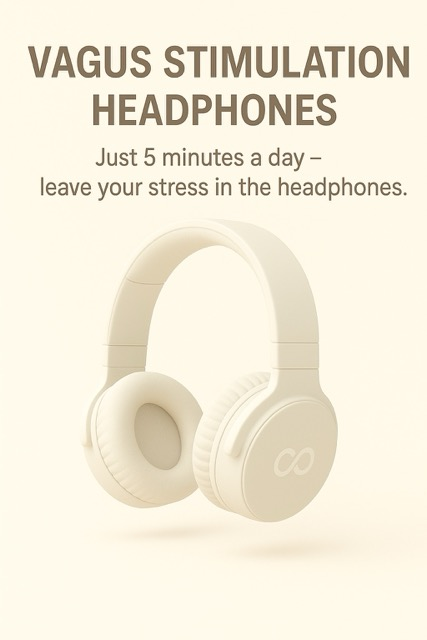
\includegraphics[keepaspectratio]{_resources/images/VNSImage Medium.jpeg}}

}

\caption{The best headphones for VNS}

\end{figure}%

\bookmarksetup{startatroot}

\chapter{Chapter 9: Integrating VNS into Daily Life: Practical
Applications and Use
Cases}\label{chapter-9-integrating-vns-into-daily-life-practical-applications-and-use-cases}

As we've explored in previous chapters, vagus nerve stimulation (VNS)
offers promising benefits for stress management, cognitive enhancement,
and sleep improvement. While the neurophysiological mechanisms and
clinical applications have been well-established, the practical
integration of VNS technology into everyday routines represents a
crucial frontier for widespread adoption. This chapter bridges the gap
between laboratory findings and real-world implementation, providing a
framework for incorporating VNS into daily activities for optimal
wellness.

\section{The Shift from Clinical to Consumer
Applications}\label{the-shift-from-clinical-to-consumer-applications}

The evolution of VNS technology from medical intervention to wellness
tool, as described in Chapter 3, has created new opportunities for
everyday applications. What was once confined to surgical implants for
epilepsy and depression treatment now includes non-invasive,
user-friendly devices designed for daily use. This democratization of
neural stimulation technology allows individuals to access its benefits
in various contexts:

\begin{itemize}
\tightlist
\item
  \textbf{Home environments}: Personal devices permit regular
  stimulation sessions without clinical supervision
\item
  \textbf{Workplace settings}: Brief interventions throughout the
  workday to manage stress and maintain focus
\item
  \textbf{Travel scenarios}: Portable solutions for mitigating
  travel-related stressors and sleep disruption
\item
  \textbf{Exercise and recovery}: Integration with physical activity
  routines for enhanced performance and recuperation
\end{itemize}

The key to effective integration is understanding not just when and how
to use VNS, but how to seamlessly incorporate it into existing routines
without adding burden or complexity.

\section{Physiological Readiness Assessment: Knowing When to
Stimulate}\label{physiological-readiness-assessment-knowing-when-to-stimulate}

Before discussing specific applications, it's important to establish how
individuals can recognize when VNS intervention might be beneficial.
Since optimal VNS effects depend on current physiological state, users
should learn to identify their autonomic balance through various
accessible indicators:

\subsection{Self-Assessment
Techniques}\label{self-assessment-techniques}

\begin{enumerate}
\def\labelenumi{\arabic{enumi}.}
\item
  \textbf{Heart rate variability awareness}: Recent research shows that
  heart rate variability (HRV) can serve as a reliable physiological
  indicator of autonomic tone during taVNS sessions\footnote{Forte et
    al. (2022)}. Studies comparing active cymba conchae stimulation with
  sham stimulation found significant increases in vagally mediated HRV
  parameters in both time and frequency domains. This suggests users can
  potentially monitor their HRV via consumer wearables to identify
  optimal times for intervention.
\item
  \textbf{Respiratory pattern observation}: Breathing rate and depth
  provide immediate feedback on autonomic state. The relationship
  between respiration and VNS efficacy is bidirectional---deep breathing
  exercises can enhance VNS effects, while VNS can improve respiratory
  regulation.
\item
  \textbf{Subjective stress scoring}: Simple self-rating of perceived
  stress on a 1-10 scale can help users decide when intervention would
  be most beneficial. This phenomenological approach, while subjective,
  correlates reasonably well with physiological stress markers.
\item
  \textbf{Physical tension inventory}: Brief body scans to identify
  muscle tension, particularly in the neck, shoulders, and jaw, can
  indicate sympathetic dominance that might benefit from vagal
  stimulation.
\end{enumerate}

Recent comparative studies by Ertürk and Özden (2025) demonstrated that
both transcutaneous auricular VNS and deep breathing exercises produced
significant decreases in perceived stress scale scores, pulse rates, and
blood pressure values after just a single session\footnote{Ertürk and
  Özden (2025)}. This supports the value of these simple physiological
measures as feedback mechanisms for timing VNS application.

\section{Daily Life Applications and Use
Cases}\label{daily-life-applications-and-use-cases}

Building on these assessment techniques, we can now explore specific
applications within the rhythms of daily life. The following scenarios
are supported by emerging research and user experience data from
consumer VNS implementations.

\subsection{Morning Routines: Starting the Day with Neural
Balance}\label{morning-routines-starting-the-day-with-neural-balance}

The transition from sleep to wakefulness represents a critical period
for establishing autonomic tone for the day ahead. Research indicates
that morning HRV patterns can predict daily stress resilience and
cognitive performance.

\textbf{Practical Application: Wake-Up Regulation}

\begin{itemize}
\tightlist
\item
  \textbf{Timing}: 5-10 minutes immediately after waking
\item
  \textbf{Device placement}: Ear-based stimulation (cymba conchae) using
  comfortable, wearable electrodes
\item
  \textbf{Protocol}: Begin with 3 minutes of low-frequency stimulation
  (3-5 Hz) to gently activate the parasympathetic system, followed by 5
  minutes of moderate frequency (15-25 Hz) to promote alertness
\item
  \textbf{Integration tips}: Combine with morning hydration routine; use
  while reviewing daily agenda
\end{itemize}

This morning protocol helps transition from the parasympathetic
dominance of sleep to balanced sympathetic activation for daytime
activities without the harsh cortisol spike associated with abrupt
awakening or alarm stress.

\subsection{Workplace Integration: Cognitive Enhancement and Stress
Management}\label{workplace-integration-cognitive-enhancement-and-stress-management}

Given the cognitive demands of modern work environments, strategic VNS
application can support both performance and wellbeing throughout the
workday.

\textbf{Practical Application: Focus Enhancement}

\begin{itemize}
\tightlist
\item
  \textbf{Timing}: Before high-concentration tasks or during attention
  slumps (typically mid-morning and mid-afternoon)
\item
  \textbf{Device option}: Neck-based or ear-based stimulation with
  discrete form factor
\item
  \textbf{Protocol}: 3-5 minutes of higher frequency stimulation (20-25
  Hz) to activate the locus coeruleus-norepinephrine system that
  supports attention
\item
  \textbf{Integration tips}: Pair with brief work breaks; schedule
  before important meetings or complex tasks
\end{itemize}

\textbf{Practical Application: Stress Recovery}

\begin{itemize}
\tightlist
\item
  \textbf{Timing}: After stressful interactions, challenging meetings,
  or intense cognitive work
\item
  \textbf{Device option}: Ear-based stimulation with comfortable earbuds
\item
  \textbf{Protocol}: 5-7 minutes of low-frequency stimulation (5-10 Hz)
  to prompt parasympathetic recovery
\item
  \textbf{Integration tips}: Combine with brief nature exposure if
  possible; use during transition periods between tasks
\end{itemize}

Studies comparing taVNS with deep breathing exercises have shown these
interventions can significantly alter autonomic measurements in favor of
parasympathetic activation\footnote{Ertürk and Özden (2025)}.
Furthermore, measurements of physical tension using myotonometry
demonstrate decreased muscle stiffness and increased relaxation
following even brief stimulation sessions---effects that are
particularly valuable in workplace settings characterized by prolonged
sitting and stress-induced muscle tension.

\subsection{Commuting and Travel: Managing Transition
Stress}\label{commuting-and-travel-managing-transition-stress}

Travel contexts present unique stressors including noise, crowding, time
pressure, and disrupted routines. VNS can provide stability during these
transitions.

\textbf{Practical Application: Commute Decompression}

\begin{itemize}
\tightlist
\item
  \textbf{Timing}: During commute or immediately upon arriving home
\item
  \textbf{Device option}: Comfortable, portable ear-based stimulator
\item
  \textbf{Protocol}: 10-15 minutes of alternating frequencies (cycling
  between low and moderate) to facilitate the transition between work
  and home mindsets
\item
  \textbf{Integration tips}: Combine with noise-cancelling functionality
  when in transit; pair with arrival rituals when reaching home
\end{itemize}

For business travelers, regular VNS sessions can help mitigate the
autonomic disruption associated with jet lag and schedule changes. Brief
stimulation periods upon wake-up in a new time zone can accelerate
circadian adjustment.

\subsection{Physical Activity Enhancement: Pre and Post-Exercise
Applications}\label{physical-activity-enhancement-pre-and-post-exercise-applications}

Exercise represents a planned stress on the autonomic system, and VNS
can optimize both performance and recovery phases.

\textbf{Practical Application: Pre-Workout Priming}

\begin{itemize}
\tightlist
\item
  \textbf{Timing}: 5-10 minutes before beginning exercise
\item
  \textbf{Device option}: Ear-based or neck-based stimulation with
  secure fit for movement
\item
  \textbf{Protocol}: Gradual increase from low to moderate frequency
  (5-15 Hz) to prepare the autonomic system for controlled stress
\item
  \textbf{Integration tips}: Incorporate during warm-up routines;
  combine with performance visualization
\end{itemize}

\textbf{Practical Application: Recovery Acceleration}

\begin{itemize}
\tightlist
\item
  \textbf{Timing}: Immediately post-exercise and/or before sleep on
  training days
\item
  \textbf{Device option}: Comfortable, stationary setup for longer
  sessions
\item
  \textbf{Protocol}: 15-20 minutes of primarily low frequency (3-8 Hz)
  stimulation to enhance parasympathetic recovery
\item
  \textbf{Integration tips}: Combine with static stretching or leisure
  reading; use during cool-down phases
\end{itemize}

Research demonstrates that alternating between deep breathing exercises
and transcutaneous VNS provides complementary benefits. In studies with
both healthy participants and those with conditions like rheumatoid
arthritis, the combination shows enhanced vagal tone as measured through
time-domain HRV parameters{[}\^{}3{]}. This suggests that integrating
both modalities into physical training regimens may offer superior
results compared to either approach alone.

\subsection{Sleep Preparation: Transitioning to Restorative
Rest}\label{sleep-preparation-transitioning-to-restorative-rest}

As discussed in Chapter 6, the relationship between VNS and sleep
quality is well-established. Practical implementation focuses on the
critical pre-sleep period.

\textbf{Practical Application: Sleep Onset Facilitation}

\begin{itemize}
\tightlist
\item
  \textbf{Timing}: 20-30 minutes before desired sleep time
\item
  \textbf{Device option}: Comfortable ear-based stimulation with minimal
  light emission
\item
  \textbf{Protocol}: 15-20 minutes of low frequency (2-5 Hz) stimulation
  with gradually decreasing intensity
\item
  \textbf{Integration tips}: Incorporate into existing bedtime routine;
  pair with reduced lighting and screen avoidance
\end{itemize}

For individuals with sleep onset difficulties, this application may
reduce the need for pharmacological interventions. The mechanism appears
to operate through both direct autonomic effects and indirect benefits
from reduced pre-sleep rumination and anxiety.

\section{Personal Customization: Building Your VNS
Protocol}\label{personal-customization-building-your-vns-protocol}

While the applications above provide starting points, effective
integration requires personalization based on individual response
patterns, lifestyle demands, and physiological baselines.

\subsection{Tracking and Adjustment
Framework}\label{tracking-and-adjustment-framework}

\begin{enumerate}
\def\labelenumi{\arabic{enumi}.}
\item
  \textbf{Establish baseline measures}: Before beginning regular VNS
  use, document typical patterns of stress, focus, sleep quality, and
  recovery using both subjective ratings and available biometric data.
\item
  \textbf{Start with standard protocols}: Begin with established
  parameters for your primary goals (stress reduction, focus
  enhancement, sleep improvement).
\item
  \textbf{Document response patterns}: Keep a simple log of:

  \begin{itemize}
  \tightlist
  \item
    Pre-stimulation state
  \item
    Protocol used (location, frequency, duration)
  \item
    Immediate post-stimulation effects
  \item
    Delayed effects (hours later)
  \end{itemize}
\item
  \textbf{Iterative refinement}: After 7-10 days, review patterns to
  identify:

  \begin{itemize}
  \tightlist
  \item
    Most effective protocols for each goal
  \item
    Optimal timing throughout the day
  \item
    Minimum effective stimulation duration
  \item
    Individual sensitivities or side effects
  \end{itemize}
\item
  \textbf{Contextual adaptation}: Adjust protocols based on seasonal
  changes, work demands, or health fluctuations.
\end{enumerate}

This personalized approach acknowledges the significant individual
variation in VNS response. Research comparing cymba conchae stimulation
with sham stimulation found that while group-level HRV increases were
significant, considerable individual variation exists in magnitude of
response\footnote{Forte et al. (2022)}. This highlights the importance
of personalized tracking rather than reliance on population averages.

\section{Multi-Modal Integration: Combining VNS with Complementary
Practices}\label{multi-modal-integration-combining-vns-with-complementary-practices}

The effectiveness of VNS can be enhanced when integrated with other
evidence-based wellness practices that target similar physiological
systems.

\subsection{Synergistic Combinations}\label{synergistic-combinations}

\begin{enumerate}
\def\labelenumi{\arabic{enumi}.}
\item
  \textbf{VNS + Breathing Practices}: Research comparing deep breathing
  exercises and transcutaneous VNS found that both interventions
  increase parasympathetic activity and promote muscle
  relaxation\textsuperscript{(Ertürk and Özden 2025)}(Jensen et al.
  2022). The combination appears particularly effective, with deep
  breathing showing superior effects on parasympathetic metrics like
  RMSSD and pNN50, while VNS demonstrated advantages in muscle
  relaxation measurements.
\item
  \textbf{VNS + Temperature Contrast}: Brief cold exposure (cold
  showers, facial immersion) activates similar vagal pathways.
  Alternating moderate cold exposure with VNS may potentiate effects.
\item
  \textbf{VNS + Music/Sound Therapy}: Acoustic stimulation with specific
  frequency profiles can enhance VNS effects on both relaxation and
  attention. Several consumer devices now offer synchronized sound and
  electrical stimulation.
\item
  \textbf{VNS + Light Exposure Management}: Coordinating VNS sessions
  with strategic light exposure (bright morning light, reduced blue
  light before sleep) can reinforce circadian regulation.
\item
  \textbf{VNS + Mindfulness Practices}: Combining taVNS with mindfulness
  meditation may create bidirectional enhancement---VNS facilitates the
  physiological state conducive to meditation, while meditation practice
  increases sensitivity to vagal effects.
\end{enumerate}

\section{Technology Solutions: Current and Emerging
Options}\label{technology-solutions-current-and-emerging-options}

A diverse ecosystem of VNS devices has emerged to support these
applications, each with advantages for specific use cases. As discussed
in Chapter 7, the hardware landscape continues to evolve, with several
categories now available:

\subsection{Key Implementation
Considerations}\label{key-implementation-considerations}

When selecting technology for daily applications, consider:

\begin{enumerate}
\def\labelenumi{\arabic{enumi}.}
\tightlist
\item
  \textbf{Form factor appropriateness}: Will the device fit comfortably
  into the intended use context?
\item
  \textbf{User control granularity}: Does the system provide adequate
  parameter adjustment?
\item
  \textbf{Feedback mechanisms}: How will you know the stimulation is
  effective?
\item
  \textbf{Battery life and charging}: Will it support your intended
  usage pattern?
\item
  \textbf{Data integration}: Can stimulation sessions be correlated with
  other health metrics?
\end{enumerate}

Particularly promising are emerging systems that adapt stimulation
parameters based on real-time physiological monitoring, creating
``closed-loop'' regulation that responds to changing conditions
throughout the day.

\section{Potential Challenges and
Solutions}\label{potential-challenges-and-solutions}

While integrating VNS into daily routines offers significant benefits,
several common challenges may arise:

\subsection{Adherence and Consistency}\label{adherence-and-consistency}

\textbf{Challenge}: Like many health practices, consistent application
can be difficult to maintain. \textbf{Solution}: Start with minimal
effective protocols; link VNS sessions to existing daily anchors
(morning coffee, commute, bedtime routine); use technology with
reminders and tracking.

\subsection{Social Acceptance}\label{social-acceptance}

\textbf{Challenge}: Using visible neurostimulation devices may draw
unwanted attention or questions. \textbf{Solution}: Select discrete form
factors for public settings; educate close contacts about the purpose
and benefits; frame as similar to other wellness technologies.

\subsection{Overstimulation Risk}\label{overstimulation-risk}

\textbf{Challenge}: Enthusiasm for benefits may lead to overuse,
potentially reducing effectiveness. \textbf{Solution}: Follow
evidence-based protocols; include ``rest days'' or reduced stimulation
periods; monitor for diminishing returns.

\subsection{Sensory Adjustment}\label{sensory-adjustment}

\textbf{Challenge}: The physical sensation of stimulation may initially
be distracting. \textbf{Solution}: Begin with lower intensity settings
and gradually increase; experiment with electrode positioning; pair
stimulation with pleasant activities to create positive associations.

\section{Conclusion: Toward Seamless
Integration}\label{conclusion-toward-seamless-integration}

As VNS technology continues to develop, the goal is increasingly
seamless integration into daily life---where neural stimulation becomes
as commonplace as other health and performance practices. The most
successful implementation approaches share certain characteristics:

\begin{enumerate}
\def\labelenumi{\arabic{enumi}.}
\tightlist
\item
  They align with natural daily rhythms and transitions
\item
  They complement rather than compete with existing routines
\item
  They provide noticeable benefits that reinforce continued use
\item
  They adapt to changing needs and contexts
\end{enumerate}

By thoughtfully applying the principles and practices outlined in this
chapter, VNS can move beyond occasional intervention to become an
integral component of daily wellness---providing ongoing support for
autonomic balance, cognitive function, and stress resilience in our
increasingly demanding world.

The next chapter will explore emerging developments in VNS technology,
including closed-loop systems and AI-enhanced protocols that promise
even more precise and personalized applications in the near future.

\bookmarksetup{startatroot}

\chapter{The Future of Neural Wellness: Closed-Loop Systems and
AI-Enhanced
VNS}\label{the-future-of-neural-wellness-closed-loop-systems-and-ai-enhanced-vns}

As we've explored throughout this book, vagus nerve stimulation (VNS)
has evolved from an invasive surgical intervention to an increasingly
accessible wellness tool. The technology continues to advance rapidly,
with emerging innovations promising to make VNS more personalized,
responsive, and intelligent. This chapter examines the future landscape
of neural wellness, with a particular focus on closed-loop VNS systems
and artificial intelligence integration that will revolutionize how we
approach mental and physical health optimization.

\section{The Limitations of Current VNS
Technology}\label{the-limitations-of-current-vns-technology}

While today's non-invasive VNS devices offer remarkable benefits, as
discussed in previous chapters, they still operate primarily as
``open-loop'' systems. This means they deliver stimulation according to
pre-programmed parameters, regardless of the user's current
physiological or psychological state. As explored in Chapter 8,
parameters like frequency, intensity, and timing can be manually
adjusted, but true dynamic responsiveness remains limited.

This one-size-fits-all approach fails to account for the significant
variability in individual responses to VNS. Some users may require more
stimulation during periods of high stress, while others might benefit
from reduced stimulation during certain activities. The effectiveness of
VNS is also known to vary with brain state, as demonstrated by Rembado
and colleagues (2021), who found that cortical responses to VNS are
modulated by different brain states (awake, resting, NREM sleep) in
non-human primates, with responses being largest during NREM
sleep\footnote{Rembado et al. (2021)}.

\section{Closed-Loop Systems: The Next Evolution in VNS
Technology}\label{closed-loop-systems-the-next-evolution-in-vns-technology}

Closed-loop VNS represents a paradigm shift from the current technology.
Rather than delivering fixed stimulation patterns, these advanced
systems continuously monitor physiological signals and adapt stimulation
parameters in real-time based on the user's current state.

\subsection{The Mechanics of Closed-Loop
VNS}\label{the-mechanics-of-closed-loop-vns}

A typical closed-loop VNS system consists of three core components:

\begin{enumerate}
\def\labelenumi{\arabic{enumi}.}
\item
  \textbf{Sensing Module}: Collects physiological data through various
  sensors monitoring biomarkers like heart rate variability (HRV),
  electrodermal activity, respiratory patterns, or even neural activity
  through EEG. Recent research by O'Grady and colleagues (2024) has
  validated the accuracy of consumer wearables like the Apple Watch for
  measuring HRV, making continuous physiological monitoring increasingly
  feasible\footnote{O'Grady et al. (2024)}.
\item
  \textbf{Processing Unit}: Analyzes incoming data to determine the
  user's current physiological and cognitive state. This component
  increasingly incorporates machine learning algorithms to detect
  patterns and predict optimal stimulation parameters.
\item
  \textbf{Adaptive Stimulation Module}: Delivers VNS with automatically
  adjusted parameters based on the processing unit's analysis, creating
  a dynamic feedback loop that continuously optimizes stimulation.
\end{enumerate}

This architecture allows the system to respond to changes in the user's
internal state, providing stimulation only when needed and at parameters
calibrated for maximum effectiveness.

\subsection{Clinical Evidence Supporting Closed-Loop
Approaches}\label{clinical-evidence-supporting-closed-loop-approaches}

Emerging research demonstrates the potential advantages of closed-loop
neuromodulation over traditional fixed-parameter approaches. Toschi and
colleagues (2023) identified causal links between brainstem responses to
transcutaneous auricular VNS (taVNS) and cardiovagal outflow, supporting
the feasibility of brainstem-targeted closed-loop stimulation for
autonomic regulation\footnote{Toschi et al. (2023)}.

In epilepsy research, studies have found that HRV-based markers can
predict seizures before they occur, suggesting the potential for VNS
systems that activate preemptively to prevent seizures. Mason et
al.~(2024) conducted a scoping review demonstrating HRV's value as a
biomarker for seizure prediction, highlighting its potential in
closed-loop intervention systems\footnote{Mason et al. (2024)}.

Perhaps most compelling is the work by Fang et al.~(2021), who developed
a machine learning model using preoperative HRV indices to predict VNS
outcomes in patients with drug-resistant epilepsy. Their model achieved
74.6\% accuracy in predicting which patients would respond to VNS
therapy, demonstrating how physiological biomarkers can inform
individualized treatment approaches\footnote{Fang et al. (2021)}.

\section{Artificial Intelligence: The Brain Behind Advanced VNS
Systems}\label{artificial-intelligence-the-brain-behind-advanced-vns-systems}

The true revolution in neural wellness will come from the integration of
artificial intelligence with VNS technology. AI systems can detect
subtle patterns in physiological data that humans might miss, predict
optimal stimulation parameters, and continuously learn from user
responses to improve effectiveness over time.

\subsection{Machine Learning for Pattern
Recognition}\label{machine-learning-for-pattern-recognition}

Machine learning algorithms can identify correlations between
physiological states and optimal VNS parameters by analyzing vast
amounts of data across users. For example, an AI system might learn that
a specific pattern of HRV fluctuation responds best to stimulation at
10Hz rather than 25Hz, or that stimulation during certain sleep phases
produces better outcomes for specific conditions.

Ding and colleagues (2019) demonstrated how machine learning approaches
using physiological data (EEG, eye tracking, and galvanic skin response)
could successfully classify depression patients and healthy controls
with 79.63\% accuracy\footnote{Ding et al. (2019)}. Similar approaches
could potentially be used to calibrate VNS parameters based on detected
mental states.

\subsection{Personalized Parameter
Optimization}\label{personalized-parameter-optimization}

Beyond pattern recognition, AI systems can develop personalized models
of individual users, accounting for their unique physiology, condition,
and response patterns. These models enable truly personalized
stimulation protocols that evolve over time as the system learns more
about the user.

Bolz and Bolz (2022) discussed the potential of evolution algorithms
that utilize device and subject data to optimize VNS parameters,
suggesting that individualized tVNS therapy could significantly improve
outcomes\footnote{Bolz and Bolz (2022)}. Such adaptive approaches
represent a substantial advancement over the manual parameter adjustment
described in Chapter 8.

\subsection{AI-Powered Companion
Applications}\label{ai-powered-companion-applications}

The integration of AI extends beyond the stimulation device itself to
companion applications that enhance the overall user experience. These
applications might include:

\begin{itemize}
\tightlist
\item
  \textbf{Virtual coaching}: AI systems that provide guidance on using
  VNS effectively and integrate it with other wellness practices
\item
  \textbf{Predictive analytics}: Tools that identify potential triggers
  or stressors before they affect the user
\item
  \textbf{Progress tracking}: Sophisticated analysis of improvements in
  targeted conditions over time
\end{itemize}

Recent research by Siddals, Torous, and Coxon (2024) explored how AI
chatbots offer mental health support that feels meaningful to
users\footnote{Siddals, Torous, and Coxon (2024)}, while Raile (2024)
examined the usefulness of ChatGPT for psychotherapists and
patients\footnote{Raile (2024)}. These studies suggest that AI
companions could enhance the therapeutic value of VNS by providing
psychological support alongside physiological intervention.

\section{Biomarker Innovation: Beyond Traditional
Measures}\label{biomarker-innovation-beyond-traditional-measures}

The effectiveness of closed-loop VNS systems depends heavily on
identifying relevant biomarkers that accurately reflect the user's
state. Future systems will likely incorporate multiple biomarkers to
create a comprehensive understanding of physiological and psychological
conditions.

\subsection{Novel Physiological
Markers}\label{novel-physiological-markers}

Beyond established measures like HRV, researchers are exploring
additional biomarkers that might provide deeper insights into neural
states:

\begin{itemize}
\tightlist
\item
  \textbf{Pupillometry}: Sharon and colleagues (2021) demonstrated that
  taVNS induces pupil dilation and attenuates alpha oscillations,
  suggesting pupil response as a potential biomarker for taVNS
  effects\footnote{Sharon, Fahoum, and Nir (2021)}.
\item
  \textbf{EEG Synchronization}: Danthine et al.~(2024) explored EEG
  synchronization measures as potential predictive biomarkers of VNS
  response in refractory epilepsy\footnote{Danthine, V., Cottin, L.,
    Berger, A., Morrison, E. I. G., Liberati, G., Santos, S. F.,
    Delbeke, J., Nonclercq, A., \& El Tahry, R. (2024).
    Electroencephalogram synchronization measure as a predictive
    biomarker of Vagus nerve stimulation response in refractory
    epilepsy: A retrospective study. PLOS ONE, 19(6), e0304115.}.
\item
  \textbf{Retinal Biomarkers}: Constable, Lim, and Thompson (2023)
  reviewed how retinal electrophysiology might serve as a ``window to
  the brain'' for central nervous system disorders\footnote{Constable,
    P. A., Lim, J. K. H., \& Thompson, D. A. (2023). Retinal
    electrophysiology in central nervous system disorders. A review of
    human and mouse studies. Frontiers in Neuroscience, 17, 1215097.}.
\end{itemize}

Pervaz and colleagues (2025) conducted a Bayesian meta-analysis
exploring the effects of different taVNS protocols on pupil dilation,
finding that pulsed stimulation protocols were significantly more
effective than continuous stimulation at inducing pupillary
changes\footnote{Pervaz, I., Thurn, L., Vezzani, C., Kaluza, L., Kühnel,
  A., \& Kroemer, N. B. (2025). Does transcutaneous auricular vagus
  nerve stimulation alter pupil dilation? A living Bayesian
  meta-analysis. Brain Stimulation, 18(2), 148-157.}. This kind of
research helps identify which biomarkers most reliably reflect the
effects of different stimulation approaches.

\subsection{Multimodal Sensing}\label{multimodal-sensing}

Future VNS systems will likely combine multiple sensing modalities to
create a more comprehensive picture of the user's state. For example, a
system might simultaneously monitor HRV, respiratory patterns, skin
conductance, and even neural activity through compact EEG sensors
embedded in everyday wearables.

The integration of multiple sensors enables more nuanced state detection
and reduces the likelihood of false positives or negatives in response
determination. For instance, Ertürk and Özden (2025) compared the acute
effects of taVNS and deep breathing exercises on autonomic nervous
system activity, demonstrating how multiple physiological measures
provide complementary insights into intervention effects\footnote{Ertürk,
  Ç., \& Özden, A. V. (2025). Comparison of the Acute Effects of
  Auricular Vagus Nerve Stimulation and Deep Breathing Exercise on the
  Autonomic Nervous System Activity and Biomechanical Properties of the
  Muscle in Healthy People. Journal of Clinical Medicine, 14(4), 1046.}.

\section{Practical Applications and Form
Factors}\label{practical-applications-and-form-factors}

The combination of closed-loop technology and AI will enable entirely
new applications and form factors for VNS, making neural wellness more
integrated into daily life.

\subsection{Next-Generation Wearables}\label{next-generation-wearables}

Future VNS devices will become increasingly discreet and comfortable,
potentially taking the form of:

\begin{itemize}
\tightlist
\item
  \textbf{Advanced Earbuds}: Building on current over-ear and in-ear
  designs, future devices might incorporate both sensing and stimulation
  capabilities in an earbud form factor indistinguishable from standard
  wireless earphones.
\item
  \textbf{Smart Jewelry}: Rings, necklaces, or bracelets that provide
  continuous monitoring and stimulation without obvious medical
  aesthetics.
\item
  \textbf{Invisible Wearables}: Ultrathin, adhesive patches or even
  temporary tattoo-like interfaces that attach directly to stimulation
  points.
\end{itemize}

As evidenced by the product materials we've examined, manufacturers are
already moving toward more consumer-friendly designs that emphasize
aesthetics and comfort alongside functionality. The development of these
form factors will be crucial for mainstream adoption of neural wellness
technology.

\subsection{Integration with Smart
Environments}\label{integration-with-smart-environments}

Beyond wearables, VNS technology may eventually integrate with smart
homes and workplaces to create environments that support neural
wellness:

\begin{itemize}
\tightlist
\item
  \textbf{Ambient Sensing}: Environmental systems that detect stress
  indicators and trigger appropriate stimulation
\item
  \textbf{Multi-Device Coordination}: Synchronization of VNS with
  lighting, sound, and other environmental factors
\item
  \textbf{Context-Aware Intervention}: Systems that understand the
  user's current activity and optimize stimulation accordingly
\end{itemize}

This level of integration would transform VNS from a discrete
intervention into a continuous, ambient support system for neural
optimization.

\section{Ethical Considerations and
Challenges}\label{ethical-considerations-and-challenges}

As with any advanced technology affecting human cognition and
physiology, next-generation VNS systems raise important ethical
questions that must be addressed:

\subsection{Data Privacy and Security}\label{data-privacy-and-security}

The extensive physiological monitoring required for closed-loop systems
creates significant privacy concerns. Users' neural and physiological
data represents highly sensitive information that could potentially
reveal detailed insights into their mental and physical health,
emotional states, and even decision-making processes.

Securing this data against unauthorized access and establishing clear
protocols for data ownership and usage will be essential as these
technologies develop. Users must maintain control over their neural data
and understand how it's being used to optimize their experience.

\subsection{Autonomy and Agency}\label{autonomy-and-agency}

As AI systems take on greater responsibility for determining stimulation
parameters, questions arise about user autonomy. To what extent should
users be able to override AI recommendations? How can systems balance
automation with user control?

Mitsea, Drigas, and Skianis (2023) explored how digitally assisted
mindfulness interventions supported by smart technologies can
effectively help develop self-regulation skills while maintaining user
agency\footnote{Mitsea, E., Drigas, A., \& Skianis, C. (2023). Digitally
  Assisted Mindfulness in Training Self-Regulation Skills for
  Sustainable Mental Health: A Systematic Review. Behavioral Sciences,
  13(12), 1008.}. Similar principles will need to be applied to
AI-enhanced VNS systems.

\subsection{Access and Equity}\label{access-and-equity}

The most advanced neural wellness technologies will likely come at
premium price points initially, potentially creating disparities in
access. Ensuring that these potentially transformative technologies
don't exacerbate existing health inequalities will require thoughtful
approaches to pricing, distribution, and even policy.

As we saw in Chapter 7, even current consumer VNS devices vary
significantly in price and accessibility, with high-end options
remaining out of reach for many potential users who might benefit from
them.

\section{The Path Forward: Interdisciplinary
Collaboration}\label{the-path-forward-interdisciplinary-collaboration}

Realizing the full potential of closed-loop, AI-enhanced VNS will
require unprecedented collaboration across disciplines:

\subsection{Neuroscience and Engineering
Partnership}\label{neuroscience-and-engineering-partnership}

Continued advancement requires deep collaboration between
neuroscientists who understand the vagus nerve's complex functions and
engineers who can develop the sensing and stimulation technologies to
interface with it effectively. The integration of these disciplines has
already driven significant innovation, as seen in the work of Wang et
al.~(2024) reviewing advances in VNS efficiency and mechanisms of action
on cognitive functions\footnote{Wang, W., Li, R., Li, C., Liang, Q., \&
  Gao, X. (2024). Advances in VNS efficiency and mechanisms of action on
  cognitive functions. Frontiers in Physiology, 15, 1452490.}.

\subsection{Clinical Validation}\label{clinical-validation}

As new technologies emerge, rigorous clinical validation will be
essential to establish efficacy, safety, and optimal use cases. The
randomized controlled trials by Wu et al.~(2022) demonstrating taVNS
effectiveness for primary insomnia\footnote{Wu, Y., Song, L., Wang, X.,
  Li, N., Zhan, S., Rong, P., Wang, Y., \& Liu, A. (2022).
  Transcutaneous Vagus Nerve Stimulation Could Improve the Effective
  Rate on the Quality of Sleep in the Treatment of Primary Insomnia: A
  Randomized Control Trial. Brain Sciences, 12(10), 1296.} and Xu et
al.~(2025) showing its benefits for depression in epilepsy
patients\footnote{Xu, Z. Y. R., Fang, J. J., Fan, X. Q., Xu, L. L., Jin,
  G. F., Lei, M. H., Wang, Y. F., Liu, J. B., Dong, F., Jiang, L. R., \&
  Guo, Y. (2025). Effectiveness and safety of transcutaneous auricular
  vagus nerve stimulation for depression in patients with epilepsy.
  Epilepsy \& Behavior, 163, 110226.} provide models for how future
technologies should be validated.

\subsection{User-Centered Design}\label{user-centered-design}

Perhaps most importantly, advancing neural wellness technology requires
deep engagement with users to understand their needs, preferences, and
experiences. As Winter et al.~(2024) explored VNS applications for
narcolepsy\footnote{Winter, Y., Sandner, K., Bassetti, C. L. A., Glaser,
  M., Ciolac, D., Ziebart, A., Karakoyun, A., Saryyeva, A., Krauss, J.
  K., Ringel, F., \& Groppa, S. (2024). Vagus nerve stimulation for the
  treatment of narcolepsy. Brain Stimulation, 17(1), 83-88.} and Yang et
al.~(2024) developed protocols for systematic evaluation of taVNS for
insomnia\footnote{Yang, T., Cai, Y., Li, X., Fang, L., \& Hu, H. (2024).
  Is transcutaneous auricular vagus nerve stimulation effective and safe
  for primary insomnia? A PRISMA-compliant protocol for a systematic
  review and meta-analysis. PLOS ONE, 19(11), e0313101.}, it becomes
clear that user experiences must guide technological development.

\section{Conclusion: The Personalized Neural Wellness
Future}\label{conclusion-the-personalized-neural-wellness-future}

The future of neural wellness through VNS technology promises a shift
from standardized interventions to highly personalized, responsive
systems that adapt to individual needs in real-time. Closed-loop systems
enhanced by artificial intelligence will transform how we understand and
optimize our own neural function, potentially addressing conditions from
anxiety and depression to cognitive performance and sleep disorders with
unprecedented precision.

As we stand at the threshold of this new era, the integration of
advanced sensing, artificial intelligence, and vagus nerve stimulation
represents not just a technological evolution but a fundamental
reconceptualization of how we approach mental and physical wellness. By
working with our nervous systems rather than merely treating their
symptoms, these technologies offer a glimpse of a future where neural
wellness becomes an integrated aspect of daily life, as accessible and
routine as physical fitness is today.

The vagus advantage of tomorrow will not merely be a technology we use,
but an intelligent system that understands and responds to our neural
needs---a true partner in the pursuit of optimal health and performance.

\bookmarksetup{startatroot}

\chapter{Summary and Conclusions}\label{summary-and-conclusions}

Throughout this book, we have explored the remarkable potential of vagus
nerve stimulation (VNS) as a tool for enhancing wellness, cognitive
performance, and physiological regulation in our increasingly demanding
world. As we conclude our journey through the science, applications, and
future of this technology, let us synthesize the key insights and
consider their implications for how we approach health and performance
optimization in modern life.

\section{The Vagus Nerve: Nature's Regulatory
Pathway}\label{the-vagus-nerve-natures-regulatory-pathway}

The vagus nerve, as we've discovered, is truly a neural highway
connecting brain and body---an elegant communication system that
influences nearly every major physiological system. This cranial nerve,
with its extensive reach from brainstem to viscera, carries
predominantly afferent (sensory) signals---about 80\% flowing from body
to brain---creating a bidirectional information superhighway that
monitors and regulates our internal state.

Through its complex network of connections, the vagus nerve: - Modulates
autonomic balance between sympathetic (``fight-or-flight'') and
parasympathetic (``rest-and-digest'') states - Influences heart rate,
respiration, digestion, and inflammation - Affects mood, attention, and
stress response through central connections to key brain regions -
Serves as a primary conduit for interoception---our sense of our body's
internal condition

This anatomical foundation helps us understand why vagal stimulation can
have such diverse effects. When we stimulate the vagus nerve, we're not
simply activating one pathway, but influencing a sophisticated network
of neural circuits that regulate multiple dimensions of our physiology
and psychology.

\section{From Clinical Treatment to Wellness
Innovation}\label{from-clinical-treatment-to-wellness-innovation}

The journey of VNS technology from invasive medical intervention to
non-invasive wellness tool illustrates how scientific discoveries can
evolve and expand beyond their original applications. Initially
developed as a surgical intervention for epilepsy and
treatment-resistant depression, VNS has transformed into a family of
non-invasive, consumer-accessible technologies.

Modern transcutaneous auricular vagus nerve stimulation (taVNS) and
cervical VNS devices now offer much of the benefit of surgical VNS
without the risks of invasive procedures. These innovations have
democratized access to neural regulation, moving from the operating room
to everyday life. By targeting accessible peripheral branches of the
vagus---particularly the auricular branch in the ear---these
technologies have made it possible to influence the same central neural
circuits through much less invasive means.

\section{The Science of Neural
Regulation}\label{the-science-of-neural-regulation}

Our exploration of the neurophysiological mechanisms behind VNS revealed
several key pathways that explain its diverse effects:

\begin{enumerate}
\def\labelenumi{\arabic{enumi}.}
\item
  \textbf{The NTS-LC-Prefrontal Pathway}: Vagal afferent signals travel
  to the nucleus tractus solitarius (NTS) in the brainstem, which then
  activates the locus coeruleus (LC). This norepinephrine-producing
  center projects to prefrontal regions, improving attention, cognitive
  function, and stress regulation.
\item
  \textbf{The Hypothalamic-Pituitary-Adrenal (HPA) Axis Regulation}: VNS
  moderates stress responses by inhibiting hypothalamic activation,
  reducing cortisol secretion, and dampening excessive physiological
  arousal.
\item
  \textbf{The Cholinergic Anti-inflammatory Pathway}: Through peripheral
  connections, vagal stimulation reduces systemic inflammation by
  modulating immune cell activity and pro-inflammatory cytokine
  production.
\item
  \textbf{The Autonomic Balance Mechanism}: VNS increases
  parasympathetic tone and heart rate variability (HRV), promoting
  physiological resilience and adaptive response to stressors.
\end{enumerate}

These mechanisms provide a scientific foundation for understanding how
VNS can simultaneously reduce stress, enhance cognition, improve sleep,
and promote overall wellness.

\section{Evidence-Based Applications}\label{evidence-based-applications}

Our review of the clinical and experimental literature has demonstrated
several well-supported applications of VNS for enhancing wellness and
performance:

\subsection{Stress and Anxiety
Management}\label{stress-and-anxiety-management}

Research consistently shows that VNS can: - Reduce cortisol levels
during acute stress challenges - Improve heart rate variability metrics
associated with stress resilience - Normalize autonomic balance in
anxiety-prone individuals - Attenuate physiological markers of stress
reactivity, such as blood pressure spikes and excessive sympathetic
activation

These effects make VNS a promising tool for managing the chronic stress
that characterizes modern professional life. By providing on-demand
access to the body's natural stress regulation systems, VNS offers a
drug-free approach to maintaining composure and equilibrium even in
high-pressure situations.

\subsection{Cognitive Enhancement}\label{cognitive-enhancement}

The cognitive benefits of VNS are particularly relevant in our
attention-challenged digital age. Studies have demonstrated that VNS
can: - Enhance sustained attention and focus, especially during fatigue
- Improve learning and memory consolidation - Increase mental clarity
and reduce cognitive fog - Support working memory and executive function

As revealed in Dr.~Robert Desimone's groundbreaking research on
attention, the brain's ability to filter relevant information from noise
depends on synchronized neural activity---a ``chorus rising above the
noise.'' VNS appears to enhance this neural synchronization,
particularly through gamma frequency oscillations that are critical for
selective attention and cognitive integration.

\subsection{Sleep and Recovery}\label{sleep-and-recovery}

In our perpetually ``on'' world, rest and recovery have become
increasingly precious. VNS has shown promising results for improving
sleep quality through several mechanisms: - Reducing sleep onset latency
and nighttime awakenings - Increasing slow-wave (deep) sleep and overall
sleep efficiency - Normalizing circadian rhythm disturbances -
Alleviating insomnia symptoms in randomized controlled trials

By promoting natural sleep architecture and parasympathetic dominance
during rest periods, VNS helps restore the recovery processes that are
fundamental to sustained cognitive and physical performance.

\section{Optimal Application: Parameters and
Protocols}\label{optimal-application-parameters-and-protocols}

As we've discussed, not all VNS is created equal. The effectiveness of
vagal stimulation depends significantly on stimulation parameters,
including:

\begin{itemize}
\tightlist
\item
  \textbf{Frequency}: Different frequency ranges produce distinct
  effects, with lower frequencies (5-10 Hz) generally promoting
  relaxation and higher frequencies (20-25 Hz) enhancing alertness and
  cognitive function.
\item
  \textbf{Intensity}: Effective stimulation requires sufficient
  intensity to activate relevant neural pathways without causing
  discomfort or adverse effects.
\item
  \textbf{Duration and Timing}: Strategic application of VNS---such as
  morning sessions for activation, midday for recovery, and evening for
  sleep preparation---maximizes benefits across different contexts.
\item
  \textbf{Location}: Ear-based (taVNS), neck-based cervical stimulation,
  and other approaches offer different advantages in terms of
  convenience, efficacy, and specificity.
\end{itemize}

Personalization emerges as a critical factor in VNS effectiveness.
Individual differences in anatomy, physiology, and response patterns
necessitate customized approaches to parameter selection and application
protocols. The future of VNS lies in adaptive, user-specific stimulation
regimens guided by real-time biofeedback.

\section{Practical Integration: VNS in Daily
Life}\label{practical-integration-vns-in-daily-life}

Perhaps the most valuable aspect of modern VNS technology is its
seamless integration into daily life. Our exploration of practical
applications revealed several key scenarios where VNS can be
strategically employed:

\begin{enumerate}
\def\labelenumi{\arabic{enumi}.}
\item
  \textbf{Morning Activation}: Using higher-frequency stimulation
  (around 25 Hz) to activate the LC-NE system, enhancing alertness and
  cognitive readiness without the jitters of caffeine.
\item
  \textbf{Post-Meeting Recovery}: Brief, lower-frequency stimulation (10
  Hz) between demanding cognitive tasks to reset stress levels and
  prevent cumulative fatigue.
\item
  \textbf{Travel Enhancement}: Moderate frequency and intermittent
  stimulation during commutes or travel to maintain mental clarity while
  managing travel-related stress.
\item
  \textbf{Lunch Break Optimization}: A biphasic approach using
  relaxation-focused stimulation followed by activation parameters to
  leverage midday breaks for true recovery and afternoon preparation.
\item
  \textbf{Evening Wind-Down}: Progressive reduction in stimulation
  frequency paired with breathing exercises to facilitate transition
  from work mode to rest.
\end{enumerate}

These practical protocols transform VNS from an abstract concept to a
concrete wellness tool that addresses the specific challenges of modern
professional life.

\section{The Future: Toward Closed-Loop Neural
Wellness}\label{the-future-toward-closed-loop-neural-wellness}

As we look forward, the most promising developments in VNS technology
involve closed-loop systems that continuously monitor physiological
state and adaptively adjust stimulation parameters based on real-time
data. These systems combine:

\begin{itemize}
\tightlist
\item
  \textbf{Multi-modal sensing} of heart rate variability, respiration,
  electrodermal activity, and other biomarkers
\item
  \textbf{Algorithmic processing} to interpret physiological patterns
  and determine optimal stimulation parameters
\item
  \textbf{Intelligent timing} that synchronizes stimulation with natural
  bodily rhythms, such as the respiratory cycle
\item
  \textbf{Personalized learning algorithms} that adapt to individual
  response patterns over time
\end{itemize}

These advances point toward a future where neural stimulation becomes
increasingly precise, personalized, and effective---responding
dynamically to changing physiological needs rather than following
static, one-size-fits-all protocols.

\section{Conclusion: The Neural
Advantage}\label{conclusion-the-neural-advantage}

In synthesizing the research, technology, and applications of vagus
nerve stimulation, we arrive at a profound conclusion: we now have the
capacity to voluntarily influence neural systems that were previously
beyond conscious control. This represents a significant advancement in
our approach to wellness and performance optimization.

VNS offers several distinct advantages over traditional approaches:

\begin{itemize}
\tightlist
\item
  \textbf{Non-pharmacological intervention} without the side effects or
  dependencies associated with medications
\item
  \textbf{Targeted physiological effects} that address root causes
  rather than merely masking symptoms
\item
  \textbf{On-demand accessibility} that allows users to respond to
  physiological needs as they arise
\item
  \textbf{Cumulative benefits} that may strengthen intrinsic regulatory
  capacities over time
\end{itemize}

These advantages position VNS as a complementary approach to traditional
health practices---not replacing sound nutrition, physical activity, and
good sleep habits, but enhancing their effects and filling gaps where
conventional approaches fall short.

The vagus advantage, ultimately, is about reclaiming agency over our
physiological state in a world that increasingly challenges our natural
regulatory capacities. By harnessing the power of neural stimulation, we
can actively participate in regulating our stress responses, cognitive
function, and recovery processes---moving from passive recipients of
modern stressors to active managers of our physiological responses.

As this technology continues to evolve, it promises to transform our
relationship with our nervous system, providing tools for navigating the
demands of modern life with greater resilience, focus, and equilibrium.
The neural revolution in wellness has only just begun, and its potential
for enhancing human flourishing in our complex world remains largely
untapped.

In closing, we invite you to consider how the principles and practices
outlined in this book might enhance your own approach to health,
performance, and well-being. The vagus advantage is not merely
theoretical---it is a practical opportunity to harness your body's
innate regulatory capacities for greater vitality and effectiveness in
all dimensions of life.

\bookmarksetup{startatroot}

\chapter{References}\label{references}

\bookmarksetup{startatroot}

\chapter*{References}\label{references-1}
\addcontentsline{toc}{chapter}{References}

\markboth{References}{References}

\phantomsection\label{refs}
\begin{CSLReferences}{1}{0}
\bibitem[\citeproctext]{ref-addorisioInvestigationalTreatmentRheumatoid2019}
Addorisio, Meghan E., Gavin H. Imperato, Alex F. De Vos, Steve Forti,
Richard S. Goldstein, Valentin A. Pavlov, Tom Van Der Poll, et al. 2019.
{``Investigational Treatment of Rheumatoid Arthritis with a Vibrotactile
Device Applied to the External Ear.''} \emph{Bioelectronic Medicine} 5
(1): 4. \url{https://doi.org/10.1186/s42234-019-0020-4}.

\bibitem[\citeproctext]{ref-alkhawajahImpactAutonomicNervous2024}
Alkhawajah, Hani A., Ali M. Y. Alshami, and Ali M. Albarrati. 2024.
{``The {Impact} of {Autonomic Nervous System Modulation} on {Heart Rate
Variability} and {Musculoskeletal Manifestations} in {Chronic Neck
Pain}: {A Double-Blind Randomized Clinical Trial}.''} \emph{Journal of
Clinical Medicine} 14 (1): 153.
\url{https://doi.org/10.3390/jcm14010153}.

\bibitem[\citeproctext]{ref-badranNeurophysiologicEffectsTranscutaneous2018}
Badran, Bashar W., Logan T. Dowdle, Oliver J. Mithoefer, Nicholas T.
LaBate, James Coatsworth, Joshua C. Brown, William H. DeVries,
Christopher W. Austelle, Lisa M. McTeague, and Mark S. George. 2018.
{``Neurophysiologic Effects of Transcutaneous Auricular Vagus Nerve
Stimulation ({taVNS}) via Electrical Stimulation of the Tragus: {A}
Concurrent {taVNS}/{fMRI} Study and Review.''} \emph{Brain Stimulation}
11 (3): 492--500. \url{https://doi.org/10.1016/j.brs.2017.12.009}.

\bibitem[\citeproctext]{ref-bolzTechnicalAspectsFuture2022}
Bolz, Armin, and Lars-Oliver Bolz. 2022. {``Technical Aspects and Future
Approaches in Transcutaneous Vagus Nerve Stimulation ({tVNS}).''}
\emph{Autonomic Neuroscience} 239 (May): 102956.
\url{https://doi.org/10.1016/j.autneu.2022.102956}.

\bibitem[\citeproctext]{ref-bremnerApplicationNoninvasiveVagal2020}
Bremner, James Douglas, Nil Z. Gurel, Matthew T. Wittbrodt, Mobashir H.
Shandhi, Mark H. Rapaport, Jonathon A. Nye, Bradley D. Pearce, et al.
2020. {``Application of {Noninvasive Vagal Nerve Stimulation} to
{Stress-Related Psychiatric Disorders}.''} \emph{Journal of Personalized
Medicine} 10 (3): 119. \url{https://doi.org/10.3390/jpm10030119}.

\bibitem[\citeproctext]{ref-bublSeeingGrayWhen2010}
Bubl, Emanuel, Elena Kern, Dieter Ebert, Michael Bach, and Ludger
Tebartz Van Elst. 2010. {``Seeing {Gray When Feeling Blue}? {Depression
Can Be Measured} in the {Eye} of the {Diseased}.''} \emph{Biological
Psychiatry} 68 (2): 205--8.
\url{https://doi.org/10.1016/j.biopsych.2010.02.009}.

\bibitem[\citeproctext]{ref-canliAmygdalaReactivityEmotional2005}
Canli, Turhan, Rebecca E. Cooney, Philippe Goldin, Maulik Shah, Heidi
Sivers, Moriah E. Thomason, Susan Whitfield-Gabrieli, John D. E.
Gabrieli, and Ian H. Gotlib. 2005. {``Amygdala Reactivity to Emotional
Faces Predicts Improvement in Major Depression.''} \emph{NeuroReport} 16
(12): 1267--70.
\url{https://doi.org/10.1097/01.wnr.0000174407.09515.cc}.

\bibitem[\citeproctext]{ref-canliBrainActivationEmotional2004}
Canli, Turhan, Heidi Sivers, Moriah E. Thomason, Susan
Whitfield-Gabrieli, John D. E. Gabrieli, and Ian H. Gotlib. 2004.
{``Brain Activation to Emotional Words in Depressed Vs Healthy
Subjects:''} \emph{NeuroReport} 15 (17): 2585--88.
\url{https://doi.org/10.1097/00001756-200412030-00005}.

\bibitem[\citeproctext]{ref-caoAccuracyAssessmentOura2022}
Cao, Rui, Iman Azimi, Fatemeh Sarhaddi, Hannakaisa Niela-Vilen, Anna
Axelin, Pasi Liljeberg, and Amir M Rahmani. 2022. {``Accuracy
{Assessment} of {Oura Ring Nocturnal Heart Rate} and {Heart Rate
Variability} in {Comparison With Electrocardiography} in {Time} and
{Frequency Domains}: {Comprehensive Analysis}.''} \emph{Journal of
Medical Internet Research} 24 (1): e27487.
\url{https://doi.org/10.2196/27487}.

\bibitem[\citeproctext]{ref-capilupiVagusNerveStimulation2020}
Capilupi, Michael J., Samantha M. Kerath, and Lance B. Becker. 2020.
{``Vagus {Nerve Stimulation} and the {Cardiovascular System}.''}
\emph{Cold Spring Harbor Perspectives in Medicine} 10 (2): a034173.
\url{https://doi.org/10.1101/cshperspect.a034173}.

\bibitem[\citeproctext]{ref-chaiFunctionalStructuralBrain2015}
Chai, Xiaoqian J., Dina Hirshfeld-Becker, Joseph Biederman, Mai Uchida,
Oliver Doehrmann, Julia A. Leonard, John Salvatore, et al. 2015.
{``Functional and Structural Brain Correlates of Risk for Major
Depression in Children with Familial Depression.''} \emph{NeuroImage:
Clinical} 8: 398--407. \url{https://doi.org/10.1016/j.nicl.2015.05.004}.

\bibitem[\citeproctext]{ref-constableRetinalElectrophysiologyCentral2023}
Constable, Paul A., Jeremiah K. H. Lim, and Dorothy A. Thompson. 2023.
{``Retinal Electrophysiology in Central Nervous System Disorders. {A}
Review of Human and Mouse Studies.''} \emph{Frontiers in Neuroscience}
17 (August): 1215097. \url{https://doi.org/10.3389/fnins.2023.1215097}.

\bibitem[\citeproctext]{ref-danthineElectroencephalogramSynchronizationMeasure2024}
Danthine, Venethia, Lise Cottin, Alexandre Berger, Enrique Ignacio
Germany Morrison, Giulia Liberati, Susana Ferrao Santos, Jean Delbeke,
Antoine Nonclercq, and Riëm El Tahry. 2024. {``Electroencephalogram
Synchronization Measure as a Predictive Biomarker of {Vagus} Nerve
Stimulation Response in Refractory Epilepsy: {A} Retrospective Study.''}
Edited by Ayataka Fujimoto. \emph{PLOS ONE} 19 (6): e0304115.
\url{https://doi.org/10.1371/journal.pone.0304115}.

\bibitem[\citeproctext]{ref-dingClassifyingMajorDepression2019}
Ding, Xinfang, Xinxin Yue, Rui Zheng, Cheng Bi, Dai Li, and Guizhong
Yao. 2019. {``Classifying Major Depression Patients and Healthy Controls
Using {EEG}, Eye Tracking and Galvanic Skin Response Data.''}
\emph{Journal of Affective Disorders} 251 (May): 156--61.
\url{https://doi.org/10.1016/j.jad.2019.03.058}.

\bibitem[\citeproctext]{ref-erturkComparisonAcuteEffects2025}
Ertürk, Çağıl, and Ali Veysel Özden. 2025. {``Comparison of the {Acute
Effects} of {Auricular Vagus Nerve Stimulation} and {Deep Breathing
Exercise} on the {Autonomic Nervous System Activity} and {Biomechanical
Properties} of the {Muscle} in {Healthy People}.''} \emph{Journal of
Clinical Medicine} 14 (4): 1046.
\url{https://doi.org/10.3390/jcm14041046}.

\bibitem[\citeproctext]{ref-fangPreoperativeHeartRate2021}
Fang, Xi, Hong-Yun Liu, Zhi-Yan Wang, Zhao Yang, Tung-Yang Cheng,
Chun-Hua Hu, Hong-Wei Hao, et al. 2021. {``Preoperative {Heart Rate
Variability During Sleep Predicts Vagus Nerve Stimulation Outcome
Better} in {Patients With Drug-Resistant Epilepsy}.''} \emph{Frontiers
in Neurology} 12 (July): 691328.
\url{https://doi.org/10.3389/fneur.2021.691328}.

\bibitem[\citeproctext]{ref-farmerInternationalConsensusBased2021}
Farmer, Adam D., Adam Strzelczyk, Alessandra Finisguerra, Alexander V.
Gourine, Alireza Gharabaghi, Alkomiet Hasan, Andreas M. Burger, et al.
2021. {``International {Consensus Based Review} and {Recommendations}
for {Minimum Reporting Standards} in {Research} on {Transcutaneous Vagus
Nerve Stimulation} ({Version} 2020).''} \emph{Frontiers in Human
Neuroscience} 14 (March): 568051.
\url{https://doi.org/10.3389/fnhum.2020.568051}.

\bibitem[\citeproctext]{ref-farrandVagusNerveStimulation2023}
Farrand, Ariana, Vincent Jacquemet, Ryan Verner, Misty Owens, and Eric
Beaumont. 2023. {``Vagus Nerve Stimulation Parameters Evoke Differential
Neuronal Responses in the Locus Coeruleus.''} \emph{Physiological
Reports} 11 (5): e15633. \url{https://doi.org/10.14814/phy2.15633}.

\bibitem[\citeproctext]{ref-forteEarYourHeart2022}
Forte, Giuseppe, Francesca Favieri, Erik Leemhuis, Maria Luisa De
Martino, Anna Maria Giannini, Luigi De Gennaro, Maria Casagrande, and
Mariella Pazzaglia. 2022. {``Ear Your Heart: Transcutaneous Auricular
Vagus Nerve Stimulation on Heart Rate Variability in Healthy Young
Participants.''} \emph{PeerJ} 10 (November): e14447.
\url{https://doi.org/10.7717/peerj.14447}.

\bibitem[\citeproctext]{ref-galinPredictivePotentialHeart2024}
Galin, Shir, and Hanna Keren. 2024. {``The {Predictive Potential} of
{Heart Rate Variability} for {Depression}.''} \emph{Neuroscience} 546
(May): 88--103.
\url{https://doi.org/10.1016/j.neuroscience.2024.03.013}.

\bibitem[\citeproctext]{ref-gencEffectsVagalNerve2024}
Genç, Ahmet, Firdevs Ezgi Uçan Tokuç, and Meltem Korucuk. 2024.
{``Effects of Vagal Nerve Stimulation Parameters on Heart Rate
Variability in Epilepsy Patients.''} \emph{Frontiers in Neurology} 15
(October): 1490887. \url{https://doi.org/10.3389/fneur.2024.1490887}.

\bibitem[\citeproctext]{ref-gotlibSubgenualAnteriorCingulate2005}
Gotlib, Ian H., Heidi Sivers, John D. E. Gabrieli, Susan
Whitfield-Gabrieli, Philippe Goldin, Kelly L. Minor, and Turhan Canli.
2005. {``Subgenual Anterior Cingulate Activation to Valenced Emotional
Stimuli in Major Depression.''} \emph{NeuroReport} 16 (16): 1731--34.
\url{https://doi.org/10.1097/01.wnr.0000183901.70030.82}.

\bibitem[\citeproctext]{ref-hartmannHeartRateVariability2019}
Hartmann, Ralf, Frank M. Schmidt, Christian Sander, and Ulrich Hegerl.
2019. {``Heart {Rate Variability} as {Indicator} of {Clinical State} in
{Depression}.''} \emph{Frontiers in Psychiatry} 9 (January): 735.
\url{https://doi.org/10.3389/fpsyt.2018.00735}.

\bibitem[\citeproctext]{ref-jensenModulatingHeartRate2022}
Jensen, Mette Kjeldsgaard, Sally Søgaard Andersen, Stine Søgaard
Andersen, Caroline Hundborg Liboriussen, Salome Kristensen, and Mads
Jochumsen. 2022. {``Modulating {Heart Rate Variability} Through {Deep
Breathing Exercises} and {Transcutaneous Auricular Vagus Nerve
Stimulation}: {A Study} in {Healthy Participants} and in {Patients} with
{Rheumatoid Arthritis} or {Systemic Lupus Erythematosus}.''}
\emph{Sensors} 22 (20): 7884. \url{https://doi.org/10.3390/s22207884}.

\bibitem[\citeproctext]{ref-jiaoEffectTranscutaneousVagus2020}
Jiao, Yue, Xiao Guo, Man Luo, Suxia Li, Aihua Liu, Yufeng Zhao, Bin
Zhao, et al. 2020. {``Effect of {Transcutaneous Vagus Nerve Stimulation}
at {Auricular Concha} for {Insomnia}: {A Randomized Clinical Trial}.''}
Edited by Francesca Mancianti. \emph{Evidence-Based Complementary and
Alternative Medicine} 2020 (1): 6049891.
\url{https://doi.org/10.1155/2020/6049891}.

\bibitem[\citeproctext]{ref-kimEffectsVagusNerve2022}
Kim, Jeong Sik, Do Eon Lee, Hyoeun Bae, Joo Yeon Song, Kwang Ik Yang,
and Seung Bong Hong. 2022. {``Effects of {Vagus Nerve Stimulation} on
{Sleep-Disordered Breathing}, {Daytime Sleepiness}, and {Sleep Quality}
in {Patients With Drug-Resistant Epilepsy}.''} \emph{Journal of Clinical
Neurology} 18 (3): 315. \url{https://doi.org/10.3988/jcn.2022.18.3.315}.

\bibitem[\citeproctext]{ref-kochMetaanalysisHeartRate2019}
Koch, Celine, Marcel Wilhelm, Stefan Salzmann, Winfried Rief, and Frank
Euteneuer. 2019. {``A Meta-Analysis of Heart Rate Variability in Major
Depression.''} \emph{Psychological Medicine} 49 (12): 1948--57.
\url{https://doi.org/10.1017/S0033291719001351}.

\bibitem[\citeproctext]{ref-kurdiIntroducingOpenAffective2017}
Kurdi, Benedek, Shayn Lozano, and Mahzarin R. Banaji. 2017.
{``Introducing the {Open Affective Standardized Image Set} ({OASIS}).''}
\emph{Behavior Research Methods} 49 (2): 457--70.
\url{https://doi.org/10.3758/s13428-016-0715-3}.

\bibitem[\citeproctext]{ref-maPreventiveNoninvasiveVagal2024}
Ma, Sai-Nan, Xiao-Hong Liu, and Wei-Song Cai. 2024. {``Preventive
Noninvasive Vagal Nerve Stimulation Reduces Insufficient Sleep-Induced
Depression by Improving the Autonomic Nervous System.''}
\emph{Biomedicine \& Pharmacotherapy} 173 (April): 116344.
\url{https://doi.org/10.1016/j.biopha.2024.116344}.

\bibitem[\citeproctext]{ref-masonHeartRateVariability2024}
Mason, Federico, Anna Scarabello, Lisa Taruffi, Elena Pasini, Giovanna
Calandra-Buonaura, Luca Vignatelli, and Francesca Bisulli. 2024.
{``Heart {Rate Variability} as a {Tool} for {Seizure Prediction}: {A
Scoping Review}.''} \emph{Journal of Clinical Medicine} 13 (3): 747.
\url{https://doi.org/10.3390/jcm13030747}.

\bibitem[\citeproctext]{ref-mitseaDigitallyAssistedMindfulness2023}
Mitsea, Eleni, Athanasios Drigas, and Charalabos Skianis. 2023.
{``Digitally {Assisted Mindfulness} in {Training Self-Regulation Skills}
for {Sustainable Mental Health}: {A Systematic Review}.''}
\emph{Behavioral Sciences} 13 (12): 1008.
\url{https://doi.org/10.3390/bs13121008}.

\bibitem[\citeproctext]{ref-nickelAnalysisSkinCorneal2024}
Nickel, Kathrin, Ludger Tebartz Van Elst, Malina Beringer, Dominique
Endres, Kimon Runge, Simon Maier, Sebastian Küchlin, et al. 2024.
{``Analysis of Skin and Corneal Fiber Electrodes for Electroretinogram
Assessments in Patients with Major Depressive Disorder.''}
\emph{Frontiers in Neuroscience} 18 (November): 1501149.
\url{https://doi.org/10.3389/fnins.2024.1501149}.

\bibitem[\citeproctext]{ref-ogradyValidityAppleWatch2024}
O'Grady, Ben, Rory Lambe, Maximus Baldwin, Tara Acheson, and Cailbhe
Doherty. 2024. {``The {Validity} of {Apple Watch Series} 9 and {Ultra} 2
for {Serial Measurements} of {Heart Rate Variability} and {Resting Heart
Rate}.''} \emph{Sensors} 24 (19): 6220.
\url{https://doi.org/10.3390/s24196220}.

\bibitem[\citeproctext]{ref-pervazDoesTranscutaneousAuricular2025}
Pervaz, Ipek, Lilly Thurn, Cecilia Vezzani, Luisa Kaluza, Anne Kühnel,
and Nils B. Kroemer. 2025. {``Does Transcutaneous Auricular Vagus Nerve
Stimulation Alter Pupil Dilation? {A} Living {Bayesian}
Meta-Analysis.''} \emph{Brain Stimulation} 18 (2): 148--57.
\url{https://doi.org/10.1016/j.brs.2025.01.022}.

\bibitem[\citeproctext]{ref-raileUsefulnessChatGPTPsychotherapists2024}
Raile, Paolo. 2024. {``The Usefulness of {ChatGPT} for Psychotherapists
and Patients.''} \emph{Humanities and Social Sciences Communications} 11
(1): 47. \url{https://doi.org/10.1057/s41599-023-02567-0}.

\bibitem[\citeproctext]{ref-redgraveSafetyTolerabilityTranscutaneous2018}
Redgrave, J., D. Day, H. Leung, P. J. Laud, A. Ali, R. Lindert, and A.
Majid. 2018. {``Safety and Tolerability of {Transcutaneous Vagus Nerve}
Stimulation in Humans; a Systematic Review.''} \emph{Brain Stimulation}
11 (6): 1225--38. \url{https://doi.org/10.1016/j.brs.2018.08.010}.

\bibitem[\citeproctext]{ref-rembadoCorticalResponsesVagus2021}
Rembado, Irene, Weiguo Song, David K Su, Ariel Levari, Larry E Shupe,
Steve Perlmutter, Eberhard Fetz, and Stavros Zanos. 2021. {``Cortical
{Responses} to {Vagus Nerve Stimulation Are Modulated} by {Brain State}
in {Nonhuman Primates}.''} \emph{Cerebral Cortex} 31 (12): 5289--5307.
\url{https://doi.org/10.1093/cercor/bhab158}.

\bibitem[\citeproctext]{ref-rongEffectTranscutaneousAuricular2016}
Rong, Peijing, Jun Liu, Liping Wang, Rupeng Liu, Jiliang Fang, Jingjun
Zhao, Yufeng Zhao, et al. 2016. {``Effect of Transcutaneous Auricular
Vagus Nerve Stimulation on Major Depressive Disorder: {A} Nonrandomized
Controlled Pilot Study.''} \emph{Journal of Affective Disorders} 195
(May): 172--79. \url{https://doi.org/10.1016/j.jad.2016.02.031}.

\bibitem[\citeproctext]{ref-sethEffectsVagusNerve2024}
Seth, Jayant, R. Grace Couper, Jorge G. Burneo, and Ana Suller Marti.
2024. {``Effects of Vagus Nerve Stimulation on the Quality of Sleep and
Sleep Apnea in Patients with Drug-Resistant Epilepsy: {A} Systematic
Review.''} \emph{Epilepsia} 65 (1): 73--83.
\url{https://doi.org/10.1111/epi.17811}.

\bibitem[\citeproctext]{ref-shaperoNeuralMarkersDepression2019}
Shapero, Benjamin G., Xiaoqian J. Chai, Mark Vangel, Joseph Biederman,
Christian S. Hoover, Susan Whitfield-Gabrieli, John D. E. Gabrieli, and
Dina R. Hirshfeld-Becker. 2019. {``Neural Markers of Depression Risk
Predict the Onset of Depression.''} \emph{Psychiatry Research:
Neuroimaging} 285 (March): 31--39.
\url{https://doi.org/10.1016/j.pscychresns.2019.01.006}.

\bibitem[\citeproctext]{ref-sharonTranscutaneousVagusNerve2021}
Sharon, Omer, Firas Fahoum, and Yuval Nir. 2021. {``Transcutaneous
{Vagus Nerve Stimulation} in {Humans Induces Pupil Dilation} and
{Attenuates Alpha Oscillations}.''} \emph{The Journal of Neuroscience}
41 (2): 320--30. \url{https://doi.org/10.1523/JNEUROSCI.1361-20.2020}.

\bibitem[\citeproctext]{ref-siddalsItHappenedBe2024}
Siddals, Steven, John Torous, and Astrid Coxon. 2024. {``{`{It} Happened
to Be the Perfect Thing'}: Experiences of Generative {AI} Chatbots for
Mental Health.''} \emph{Npj Mental Health Research} 3 (1): 48.
\url{https://doi.org/10.1038/s44184-024-00097-4}.

\bibitem[\citeproctext]{ref-toschiCausalInfluenceBrainstem2023}
Toschi, Nicola, Andrea Duggento, Riccardo Barbieri, Ronald G. Garcia,
Harrison P. Fisher, Norman W. Kettner, Vitaly Napadow, and Roberta
Sclocco. 2023. {``Causal Influence of Brainstem Response to
Transcutaneous Vagus Nerve Stimulation on Cardiovagal Outflow.''}
\emph{Brain Stimulation} 16 (6): 1557--65.
\url{https://doi.org/10.1016/j.brs.2023.10.007}.

\bibitem[\citeproctext]{ref-wangAdvancesVNSEfficiency2024}
Wang, Wendi, Rui Li, Chuangtao Li, Qimin Liang, and Xiaolin Gao. 2024.
{``Advances in {VNS} Efficiency and Mechanisms of Action on Cognitive
Functions.''} \emph{Frontiers in Physiology} 15 (October): 1452490.
\url{https://doi.org/10.3389/fphys.2024.1452490}.

\bibitem[\citeproctext]{ref-winterVagusNerveStimulation2024}
Winter, Yaroslav, Katharina Sandner, Claudio L. A. Bassetti, Martin
Glaser, Dumitru Ciolac, Andreas Ziebart, Ali Karakoyun, et al. 2024.
{``Vagus Nerve Stimulation for the Treatment of Narcolepsy.''}
\emph{Brain Stimulation} 17 (1): 83--88.
\url{https://doi.org/10.1016/j.brs.2024.01.002}.

\bibitem[\citeproctext]{ref-woodhamHomebasedTranscranialDirect2025}
Woodham, Rachel D., Sudhakar Selvaraj, Nahed Lajmi, Harriet Hobday,
Gabrielle Sheehan, Ali-Reza Ghazi-Noori, Peter J. Lagerberg, et al.
2025. {``Home-Based Transcranial Direct Current Stimulation Treatment
for Major Depressive Disorder: A Fully Remote Phase 2 Randomized
Sham-Controlled Trial.''} \emph{Nature Medicine} 31 (1): 87--95.
\url{https://doi.org/10.1038/s41591-024-03305-y}.

\bibitem[\citeproctext]{ref-wuTranscutaneousVagusNerve2022}
Wu, Yating, Lu Song, Xian Wang, Ning Li, Shuqin Zhan, Peijing Rong,
Yuping Wang, and Aihua Liu. 2022. {``Transcutaneous {Vagus Nerve
Stimulation Could Improve} the {Effective Rate} on the {Quality} of
{Sleep} in the {Treatment} of {Primary Insomnia}: {A Randomized Control
Trial}.''} \emph{Brain Sciences} 12 (10): 1296.
\url{https://doi.org/10.3390/brainsci12101296}.

\bibitem[\citeproctext]{ref-xuEffectivenessSafetyTranscutaneous2025}
Xu, Zheng Yan Ran, Jia Jia Fang, Xiao Qin Fan, Long Long Xu, Gui Fang
Jin, Mei Hua Lei, Yu Fei Wang, et al. 2025. {``Effectiveness and Safety
of Transcutaneous Auricular Vagus Nerve Stimulation for Depression in
Patients with Epilepsy.''} \emph{Epilepsy \& Behavior} 163 (February):
110226. \url{https://doi.org/10.1016/j.yebeh.2024.110226}.

\bibitem[\citeproctext]{ref-yakuninaOptimizationTranscutaneousVagus2017}
Yakunina, Natalia, Sam Soo Kim, and Eui-Cheol Nam. 2017. {``Optimization
of {Transcutaneous Vagus Nerve Stimulation Using Functional MRI}.''}
\emph{Neuromodulation: Technology at the Neural Interface} 20 (3):
290--300. \url{https://doi.org/10.1111/ner.12541}.

\bibitem[\citeproctext]{ref-yangTranscutaneousAuricularVagus2024}
Yang, Ting, Yunhuo Cai, Xingling Li, Lianqiang Fang, and Hantong Hu.
2024. {``Is Transcutaneous Auricular Vagus Nerve Stimulation Effective
and Safe for Primary Insomnia? {A PRISMA-compliant} Protocol for a
Systematic Review and Meta-Analysis.''} Edited by Yung-Hsiang Chen.
\emph{PLOS ONE} 19 (11): e0313101.
\url{https://doi.org/10.1371/journal.pone.0313101}.

\bibitem[\citeproctext]{ref-zhangEffectsTranscutaneousAuricular2021}
Zhang, Shuai, Jia-Kai He, Hong Meng, Bin Zhao, Ya-Nan Zhao, Yu Wang,
Shao-Yuan Li, et al. 2021. {``Effects of Transcutaneous Auricular Vagus
Nerve Stimulation on Brain Functional Connectivity of Medial Prefrontal
Cortex in Patients with Primary Insomnia.''} \emph{The Anatomical
Record} 304 (11): 2426--35. \url{https://doi.org/10.1002/ar.24785}.

\end{CSLReferences}


\backmatter

\printindex


\end{document}
